
In this supplementary material, we first provide implementation details of our try-on condition generator, and then present the additional qualitative results.
Lastly, we compare the number of learnable parameters and inference times between methods.
Since there are many qualitative results, we recommend not to print this material.

\section{Implementation Details}
We implement our proposed method on top of the official PyTorch implementation of HR-VITON~\cite{lee2022hrviton}.
Our implementation details are the same with HR-VITON.
Specifically, we set the batch sizes to $8$ when training our try-on condition generator.
The learning rate is set to $0.0002$. 
We train our model until $100,000$ iterations.
The training and inference strategies are also the same with HR-VITON.
During the training phase, our try-on condition generator predicts the segmentation map~($\hat{S}$), the warped clothes~($\hat{I}_c$), and the warped clothes mask~($\hat{S}_c$), each of which has $256 \times 192$ resolution.
In the inference stage, the appearance flow map~($F$) and $\hat{S}$ are upscaled to $1024 \times 768$ resolution.
Thus, $\hat{S}$, $\hat{I}_c$, and $\hat{S}_c$ with $1024 \times 768$ resolution are given to our try-on image generator.

\begin{figure}[t]
	\centering
    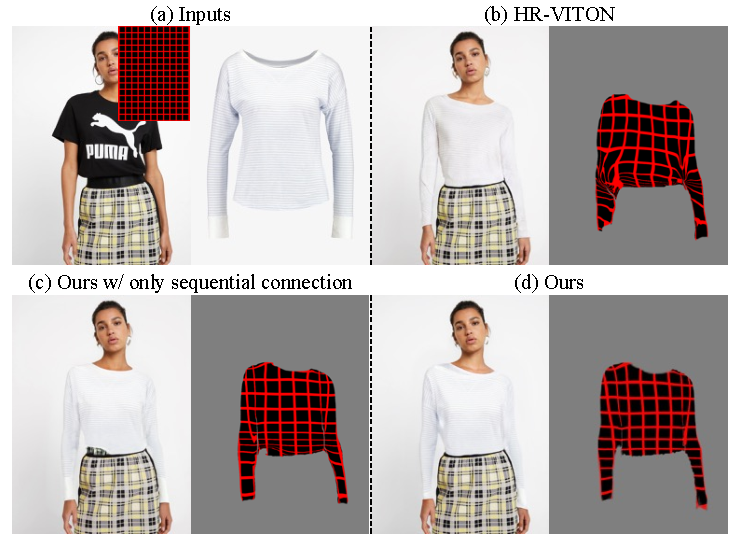
\includegraphics[width=\linewidth]{fig_supp/fig8.pdf}    
    \caption{Visualization of a try-on sample and a warped grid. (b) The warped grid of HR-VITON is squeezed nearby the sleeve and the waist. (c) Our ablated model produces a warped grid without squeezing around the sleeve, but the grid is progressively narrowed around the waist. (d) Ours full model deforms a grid without any squeezing problem.}
	\label{fig_warped_grid}
\end{figure}


\section{More Qualitative Results}


\paragraph{Visualization of warped grid.} 
Given a grid image, Fig.~\ref{fig_warped_grid} shows a comparison of warped grid between different methods.
The warped grid of HR-VITON is squeezed nearby the arm and waist.
On the other hands, ours w/ sequential connection does not have a squeezed grid on the arm.
However, we observe that the area of grid gradually shrinks nearby the waist.
This result implies that the model decided to deform clothes with preserving the whole contents with squeezed textures.
Lastly, our full model successfully removes the partial contents of clothes and has a consistent interval between grids.
These results confirm that our proposed methods successfully address our raised two types of squeezing artifacts.

\paragraph{Generated samples for persons with tucked-out shirts style and clothes with short- or no sleeves} are reported in Fig.~\ref{fig_supp_causal}.
As seen in the results, the visual quality of generated samples is indistinguishable between ours and HR-VITON~\cite{lee2022hrviton}.
This shows that our proposed method does not degrade the visual quality
even for the configuration different from our main subject, 
clothes with long sleeves or a person with a tucked-in shirts style.

\paragraph{Sleeve-squeezing artifact.}
Fig.~\ref{fig_supp_longsleeve} shows the comparison of generated samples when clothes with long sleeves are given.
In most tested cases, HR-VITON suffers from the sleeve-squeezing artifact.
On the other hand, our method successfully generates the samples by preserving the unique textures of clothes on arms.
Additional high-resolution qualitative results are available in Fig.~\ref{fig_supp_longsleeve_HR_0} -- \ref{fig_supp_longsleeve_HR_5}.


\paragraph{Waist-squeezing artifact.}
We also report the qualitative comparison with respect to waist-squeezing artifacts.
As shown in Fig.~\ref{fig_supp_tucked_in}, HR-VITON generates the samples with preserving the whole contents with a squeezed texture nearby a waist.
On the other hand, our method produces the samples without squeezed texture around the waist, since our model is able to erase the partial contents of clothes.
More high-resolution qualitative results are presented in Fig.~\ref{fig_supp_tucked_in_HR_6} -- \ref{fig_supp_tucked_in_HR_11}.


\begin{table}[t]
	\centering
	\begin{tabular}{l|c|c}
		\toprule
		Methods  & \#Params of Gs & Frames per second \\
		\midrule
		\midrule
        VITON-HD  & 154.07M & N/A \\
        HR-VITON  & \textbf{147.91M} &  \textbf{2.49} \\
        Ours & 148.14M & \textbf{2.49} \\
		\bottomrule
	\end{tabular}
    \caption{Number of parameters and inference time.
    }
	\label{tb_computational_costs}
\end{table}


\section{Number of Parameters and Inference Time}
\paragraph{Number of learnable parameters} are reported in Table.~\ref{tb_computational_costs}. Since our methods only require an additional 3D convolution operation at the last fusion block, the increment of learnable parameters is $0.23$ million than HR-VITON.
It clarifies that our improvement is not caused by increasing the model capacity. 

\paragraph{Inference times} are compared by measuring the frames-per-second~(FPS) of HR-VITON and Ours. Note that, the batch size is set to $1$ when measuring times. As reported in Table.~\ref{tb_computational_costs}, the inference times are nearly identical (2.49 FPS) on a single A6000 GPU.


\begin{figure*}[t!]
    \centering
     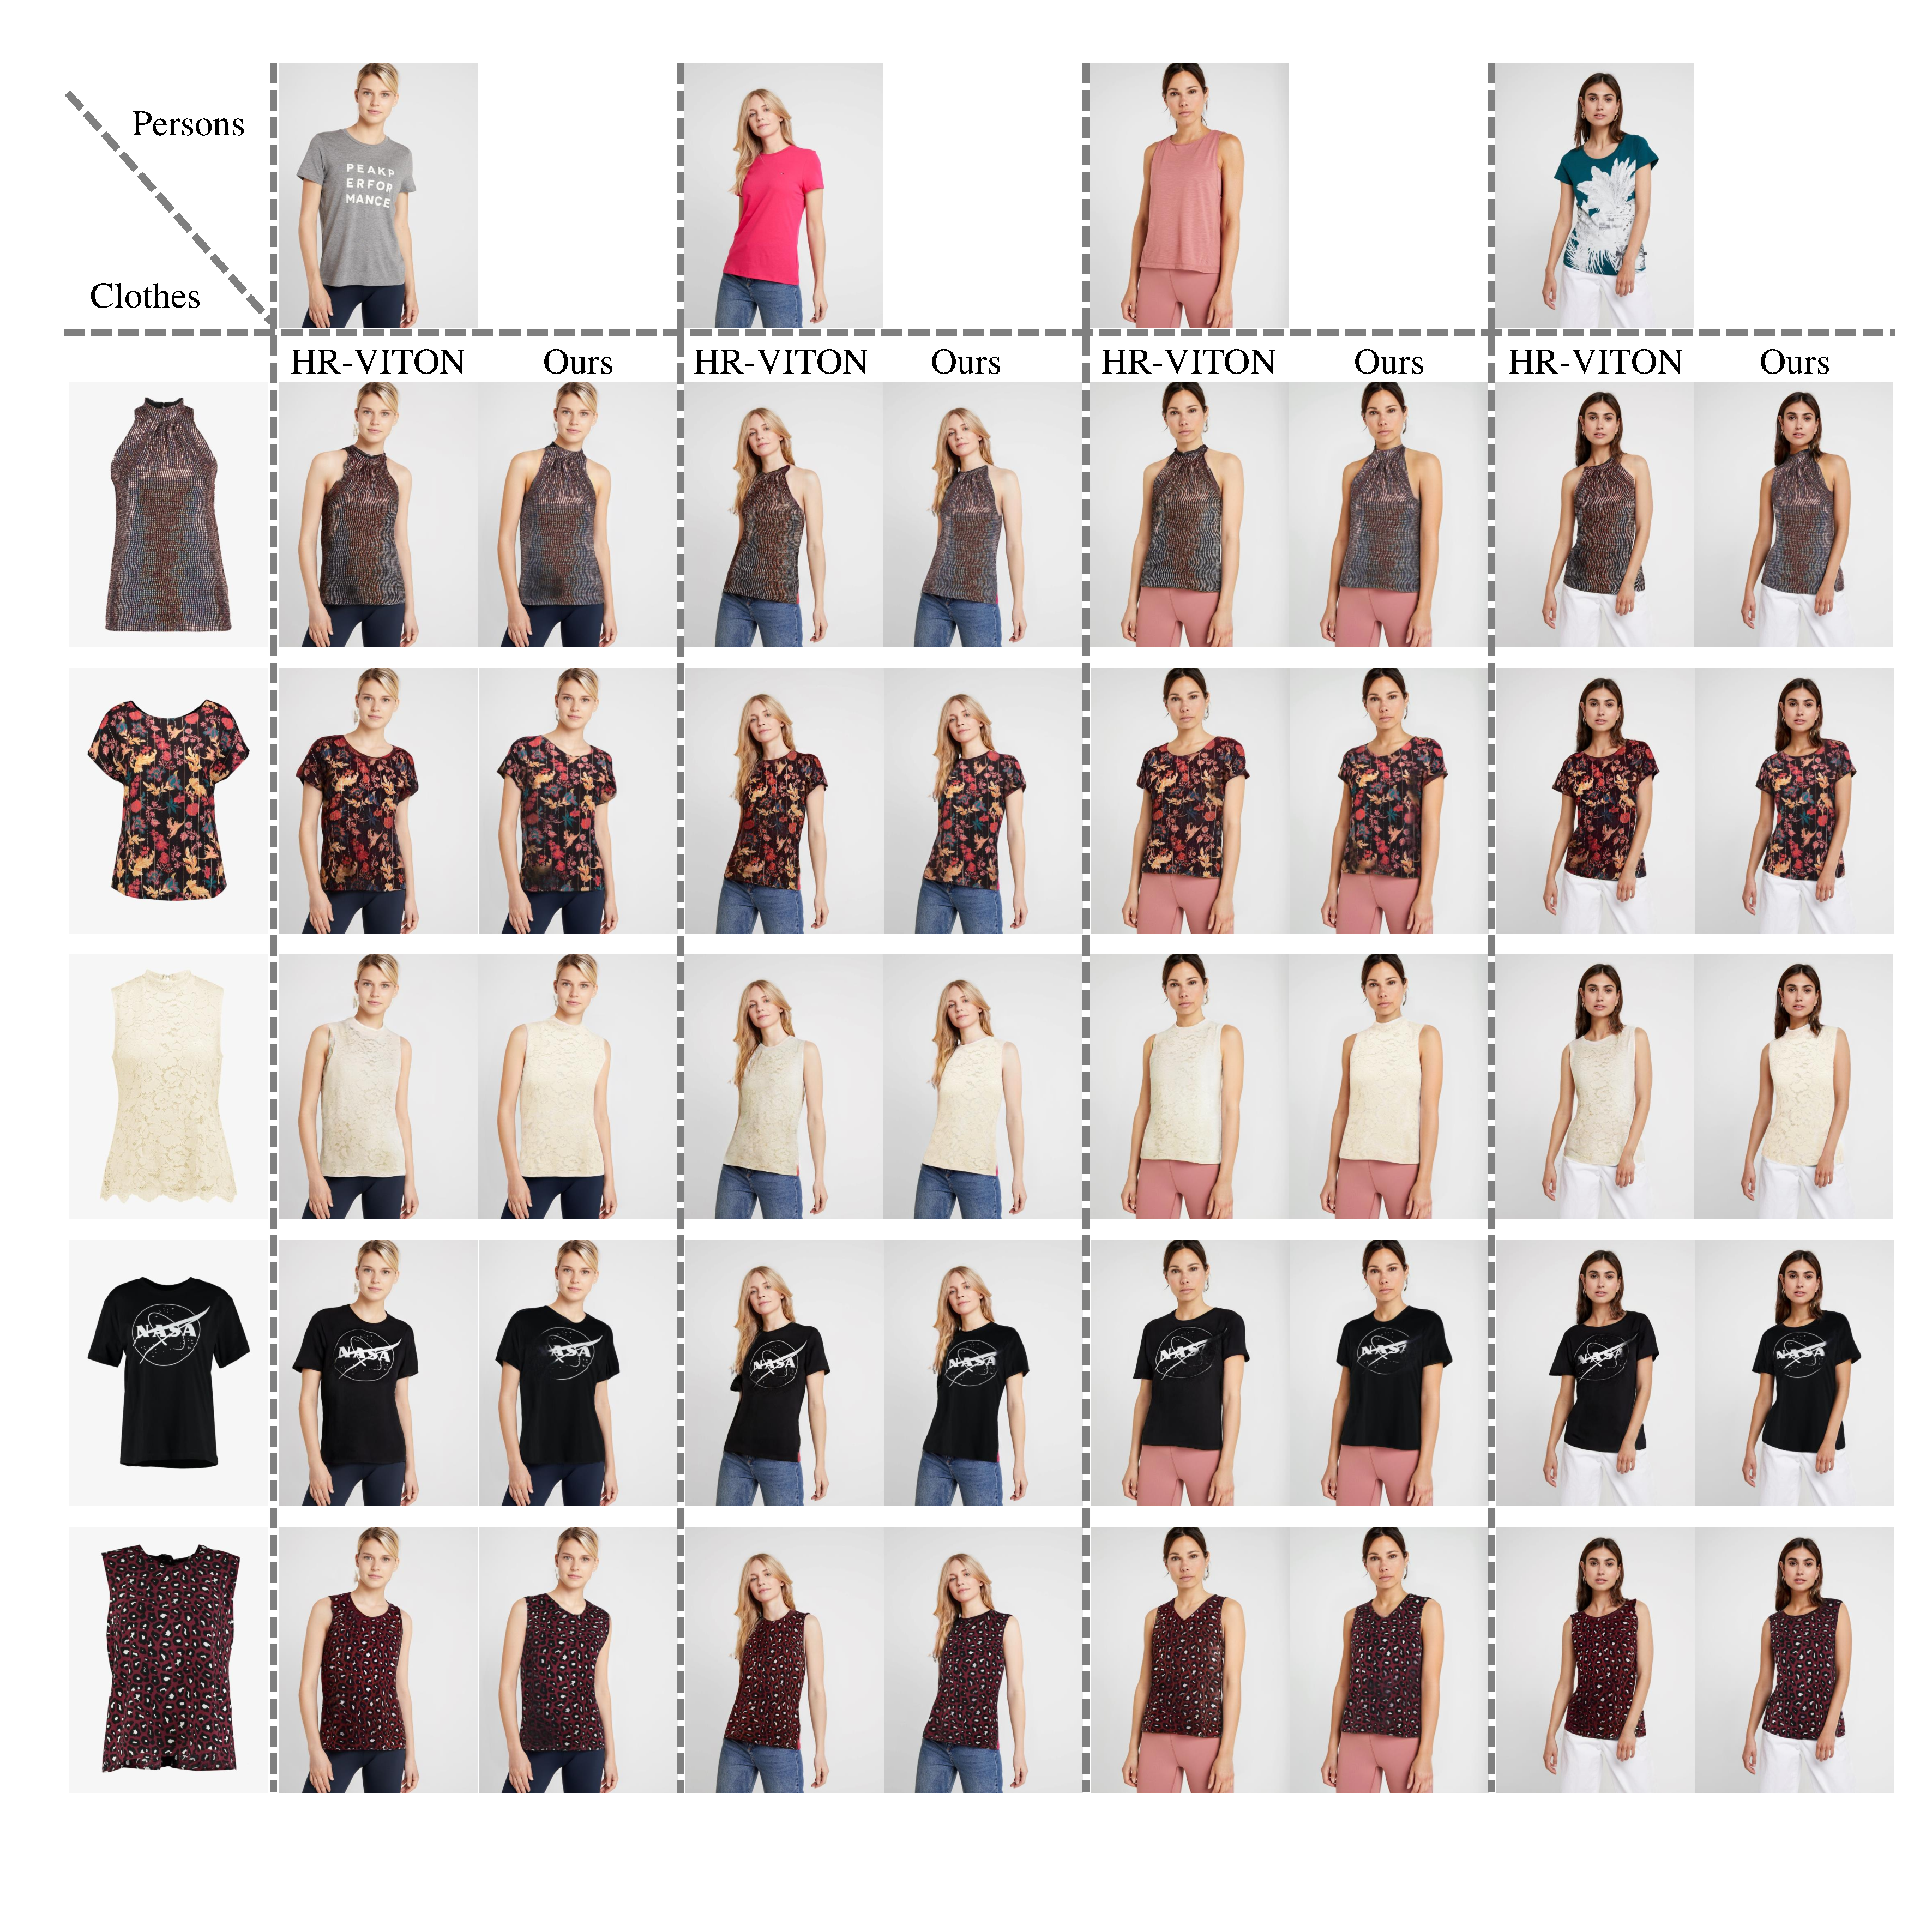
\includegraphics[width=\textwidth]{fig_supp/fig_supp_causal.pdf}
     \caption{Qualitative comparison between HR-VITON~\cite{lee2022hrviton} and ours. The input pair is the person with a tucked-out shirts style and the clothes with short- or no sleeves which are not our main concern. For those pairs, the visual quality of generated samples is indistinguishable between the baseline and ours. These results show that our proposed method does not degrade the performance even for the configuration different from our main subject in this paper.
     \label{fig_supp_causal}
     }
\end{figure*}

\begin{figure*}[t!]
    \centering
     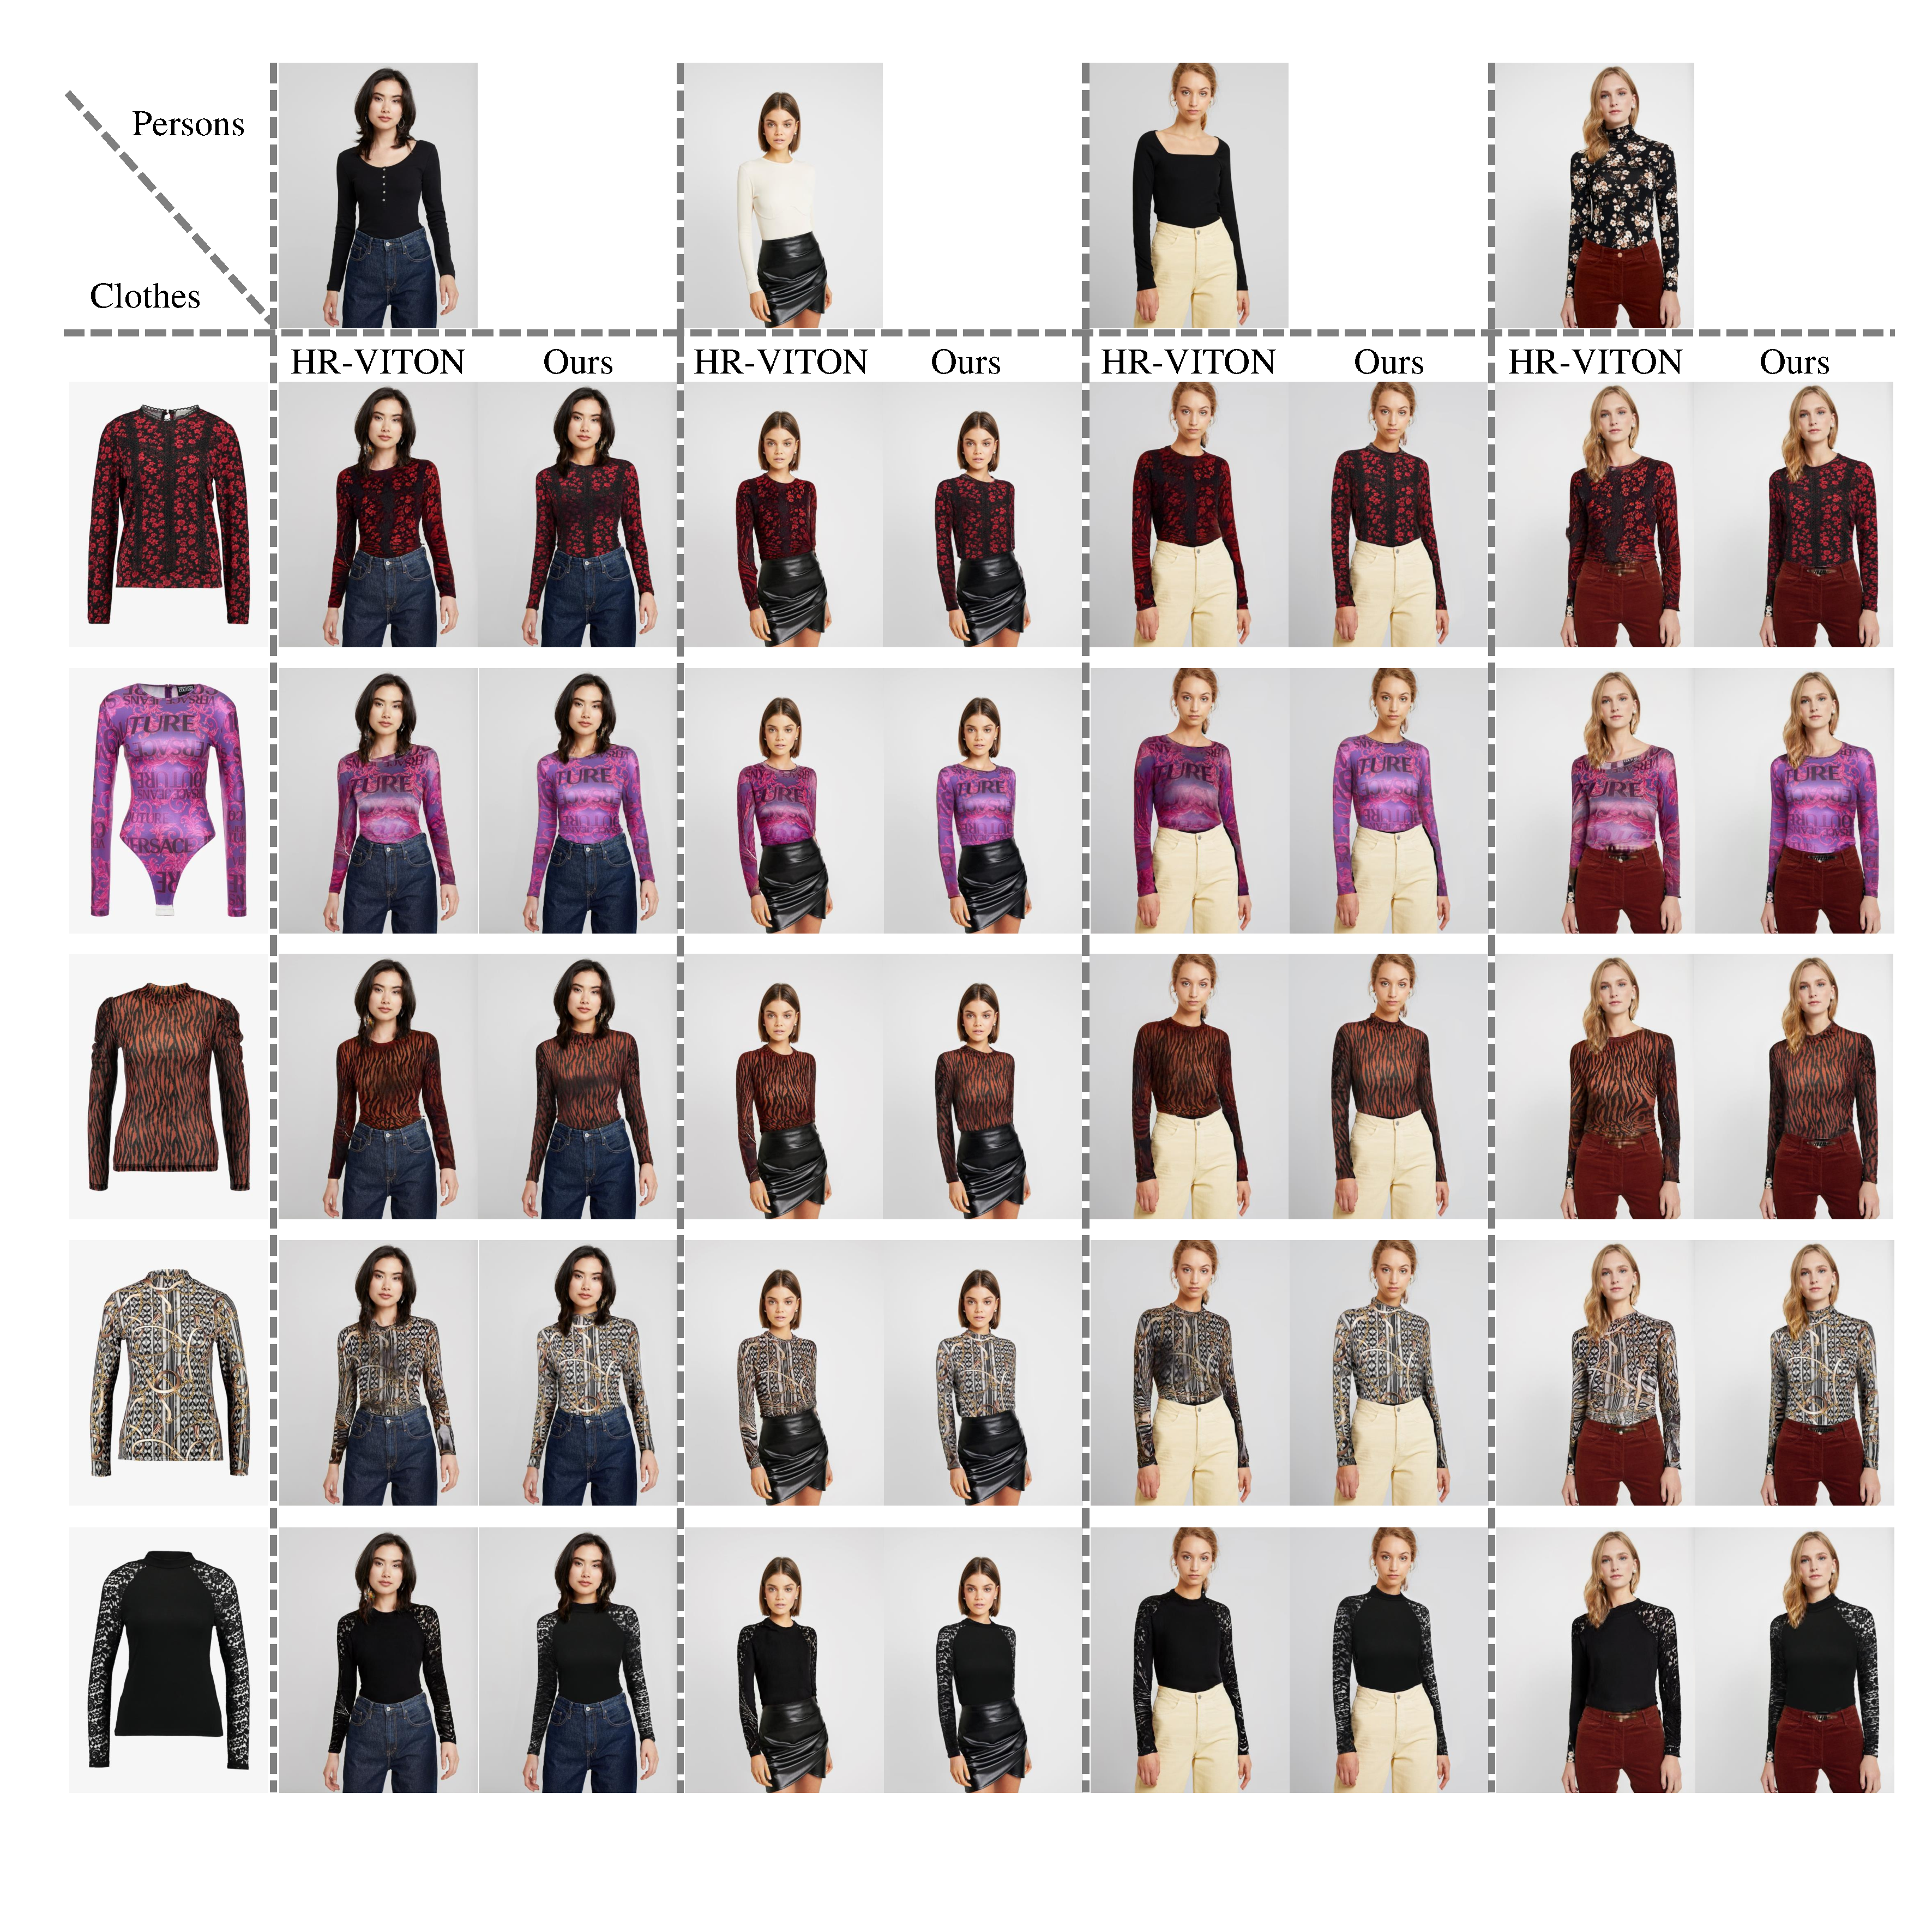
\includegraphics[width=\textwidth]{fig_supp/fig_supp_longsleeve.pdf}
     \caption{Qualitative comparison between HR-VITON~\cite{lee2022hrviton} and ours. We recommend to look into the arm. Most generated samples from HR-VITON have squeezed textures on arm, whereas the synthesized samples from our model have the unique clothing texture on arm.
     }
     \label{fig_supp_longsleeve}
\end{figure*}

\begin{figure*}[t!]
    \centering
     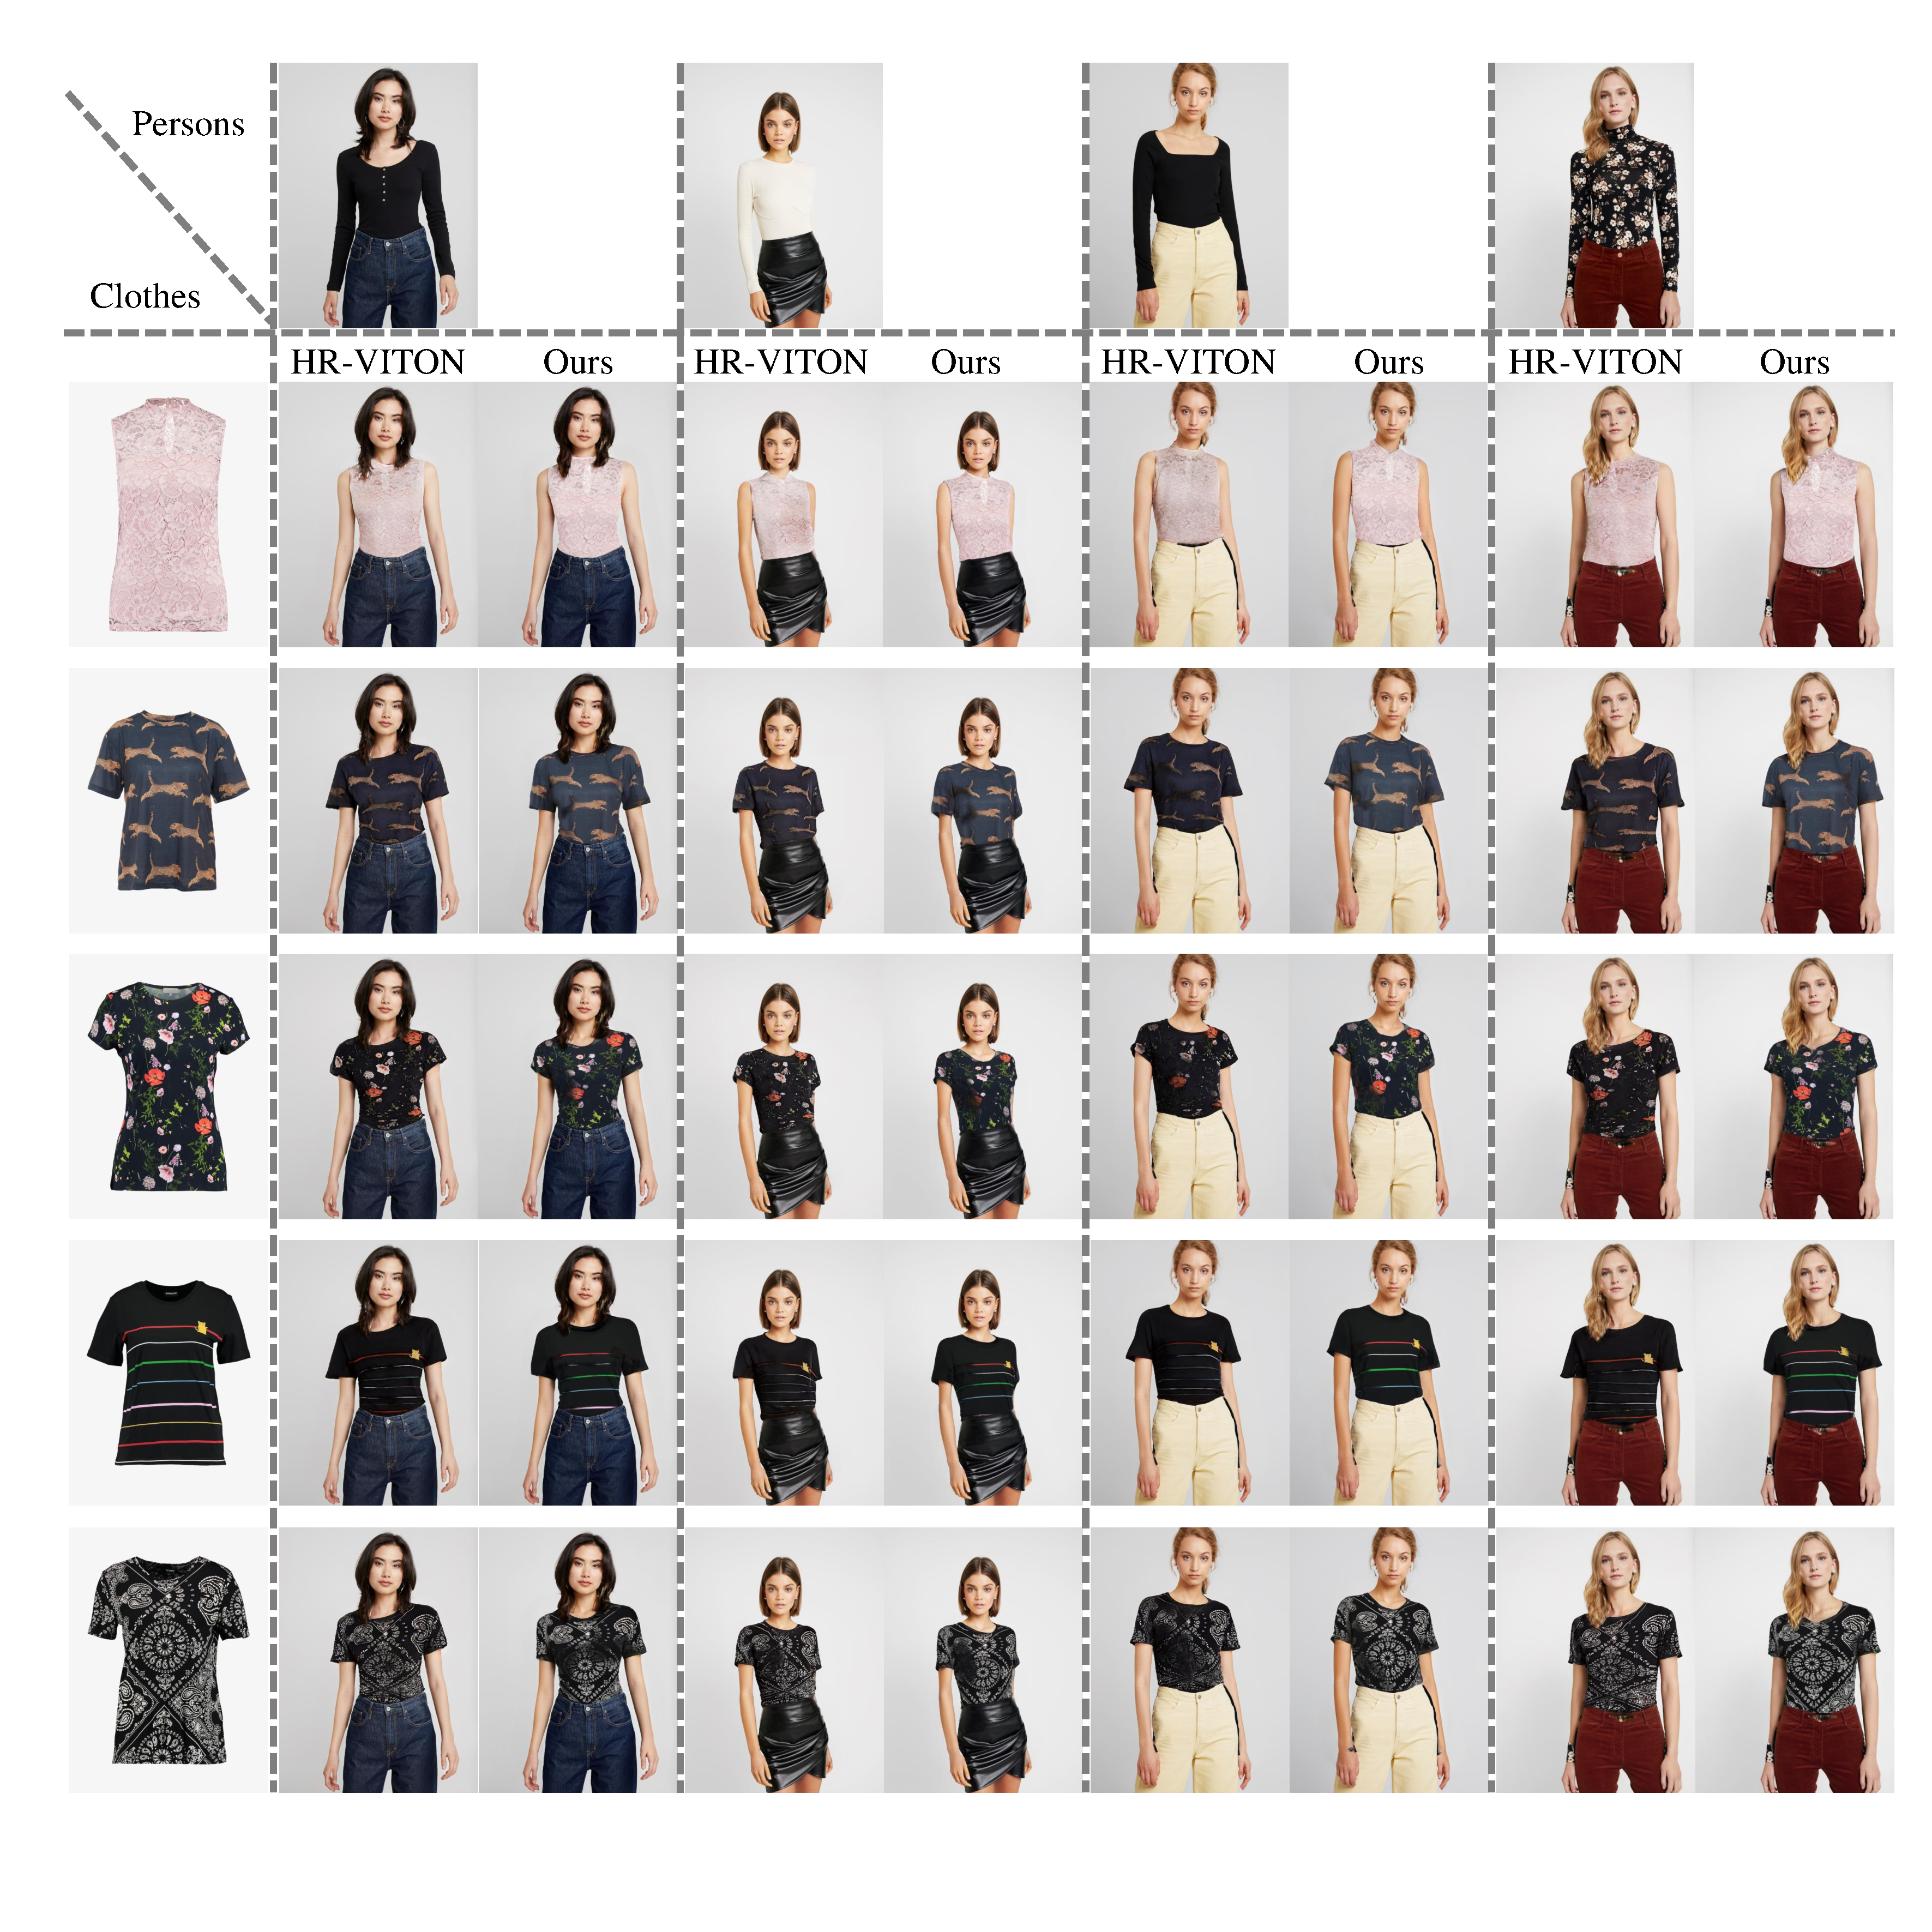
\includegraphics[width=\textwidth]{fig_supp/fig_supp_tucked_in.pdf}
     \caption{Qualitative comparison between HR-VITON~\cite{lee2022hrviton} and ours. We recommend to look into the waist. The baseline produces the samples with preserving the whole contents with squeezed textures, while our model generates the samples without squeezed textures nearby the waist since our model is able to erase the partial contents of clothes.
     }
     \label{fig_supp_tucked_in}
\end{figure*}

\begin{figure*}[t!]
    \centering
     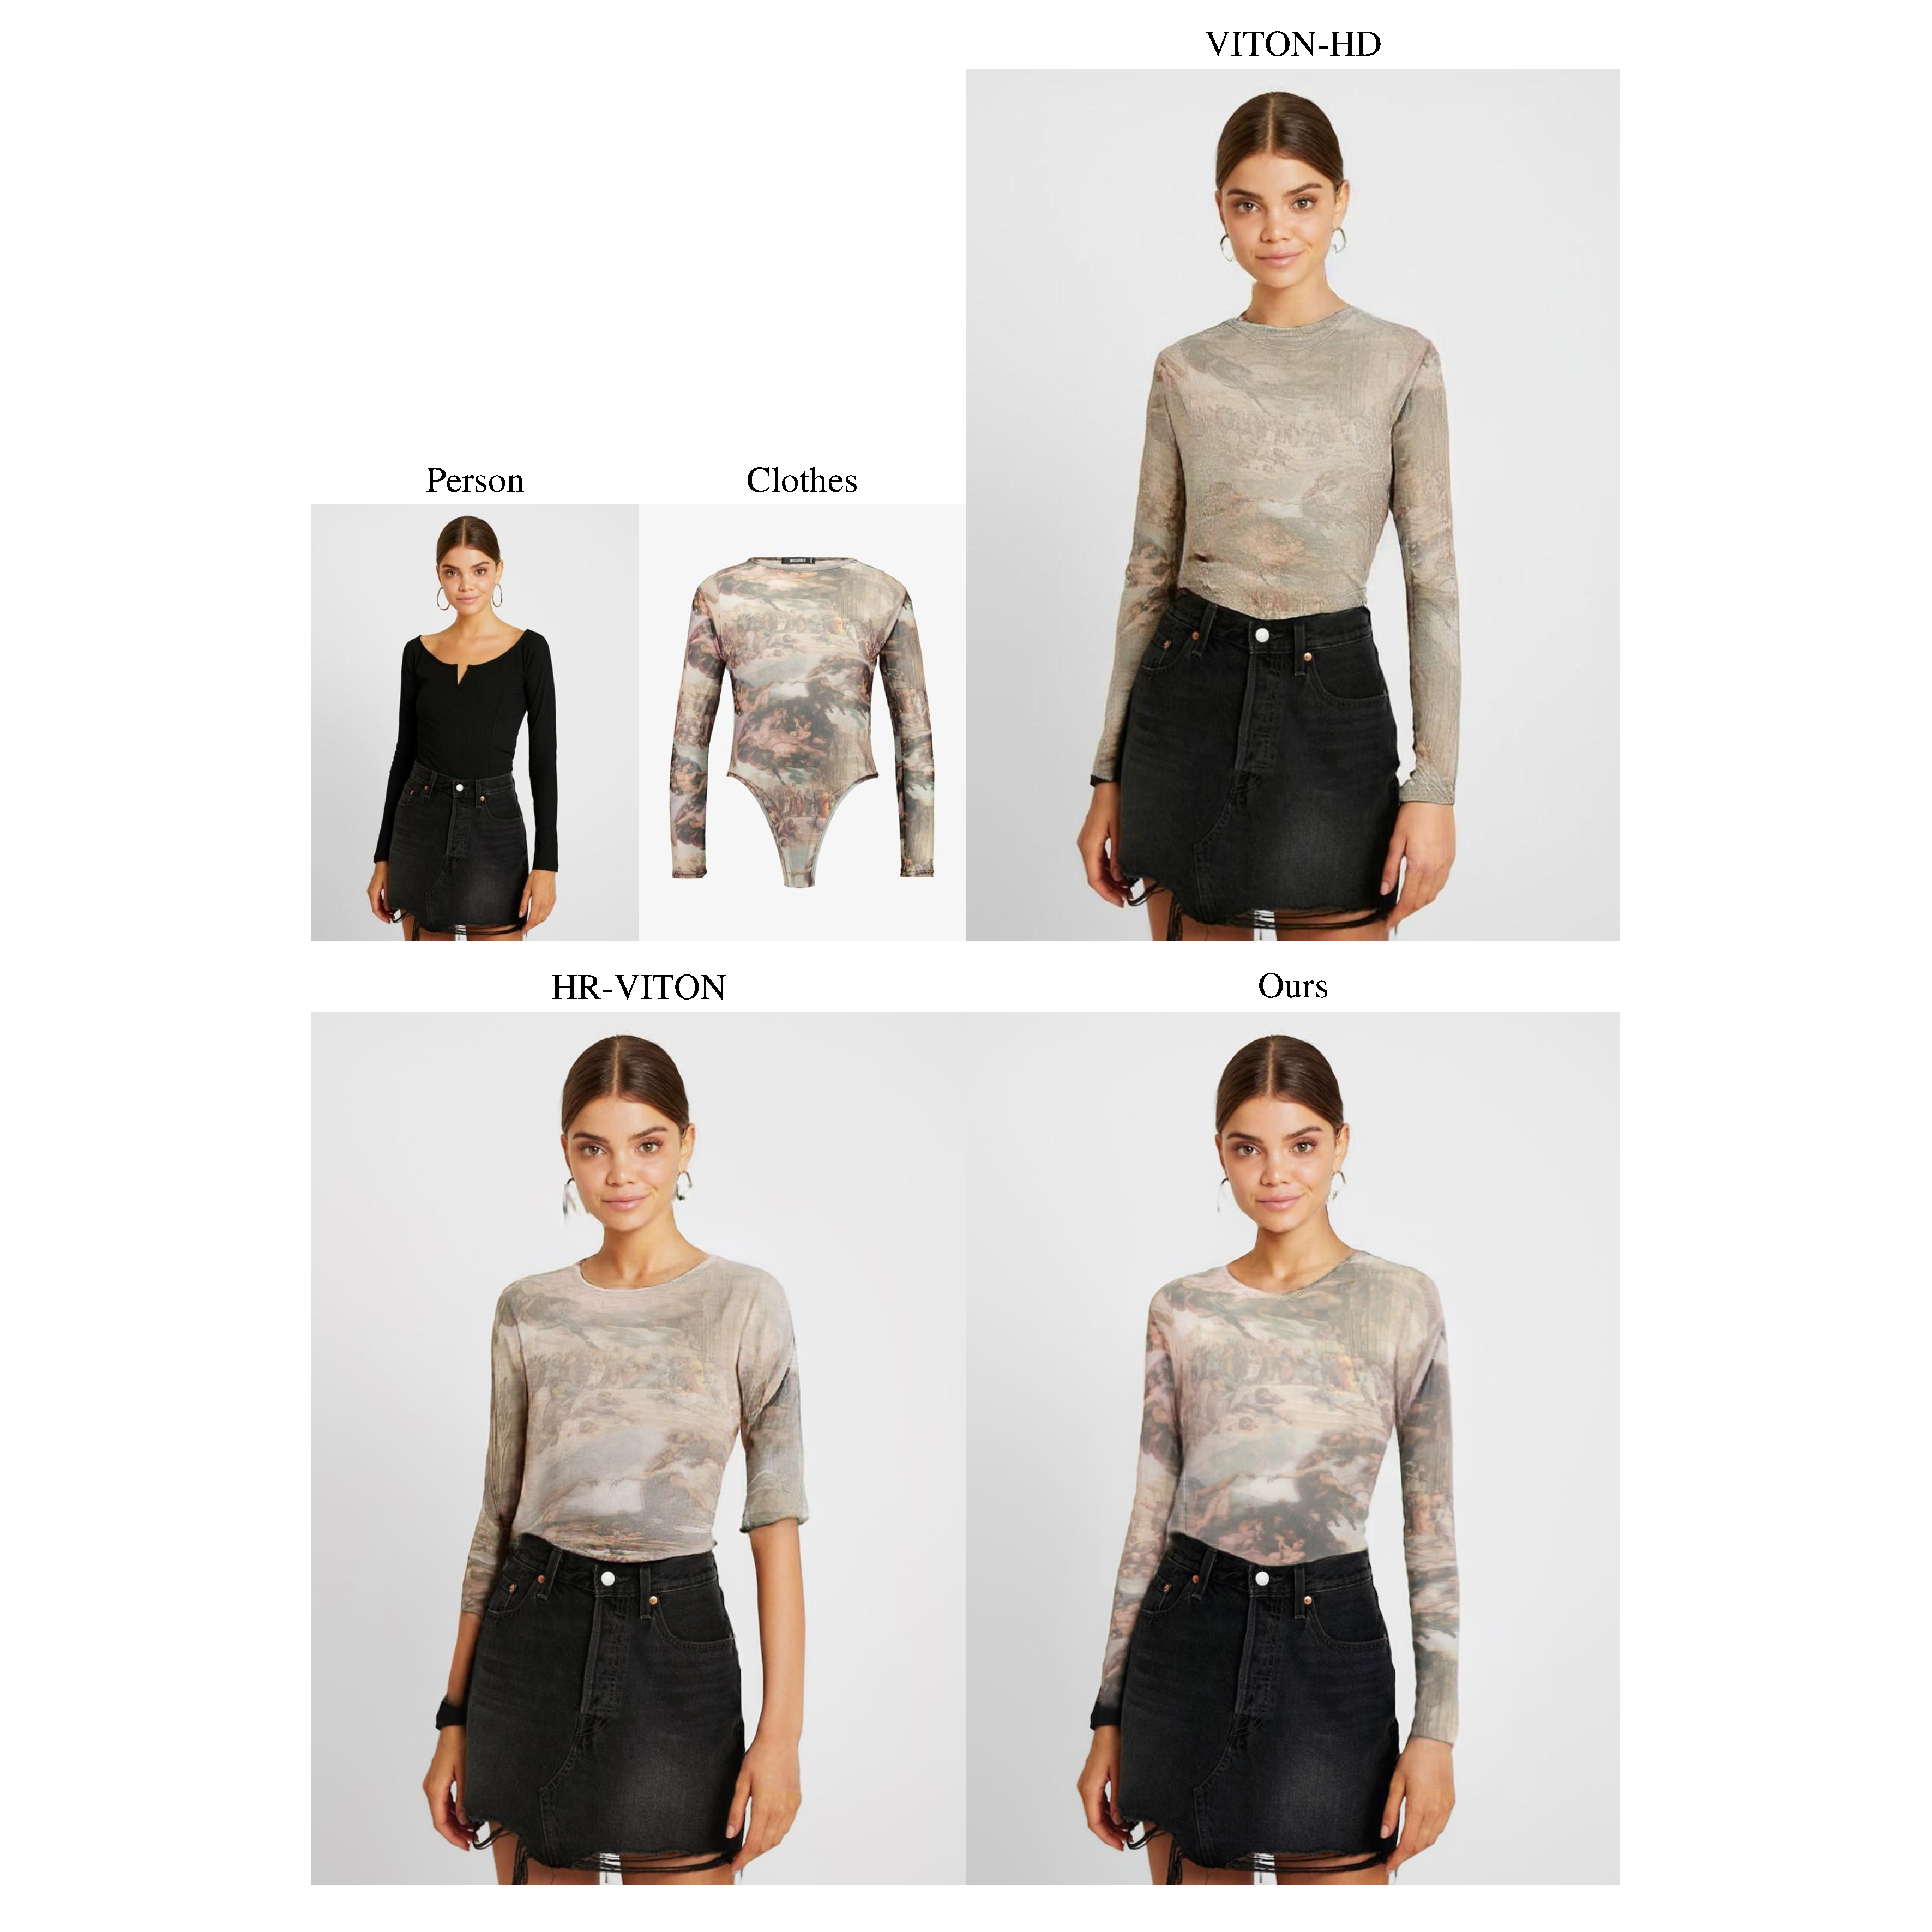
\includegraphics[width=0.85\textwidth]{fig_supp/fig_suppl_HD_3.pdf}
     \caption{Qualitative comparison between VITON-HD~\cite{choi2021viton}, HR-VITON~\cite{lee2022hrviton}, and ours. We recommend to look into the arm.
     }
     \label{fig_supp_longsleeve_HR_0}
\end{figure*}

\begin{figure*}[t!]
    \centering
     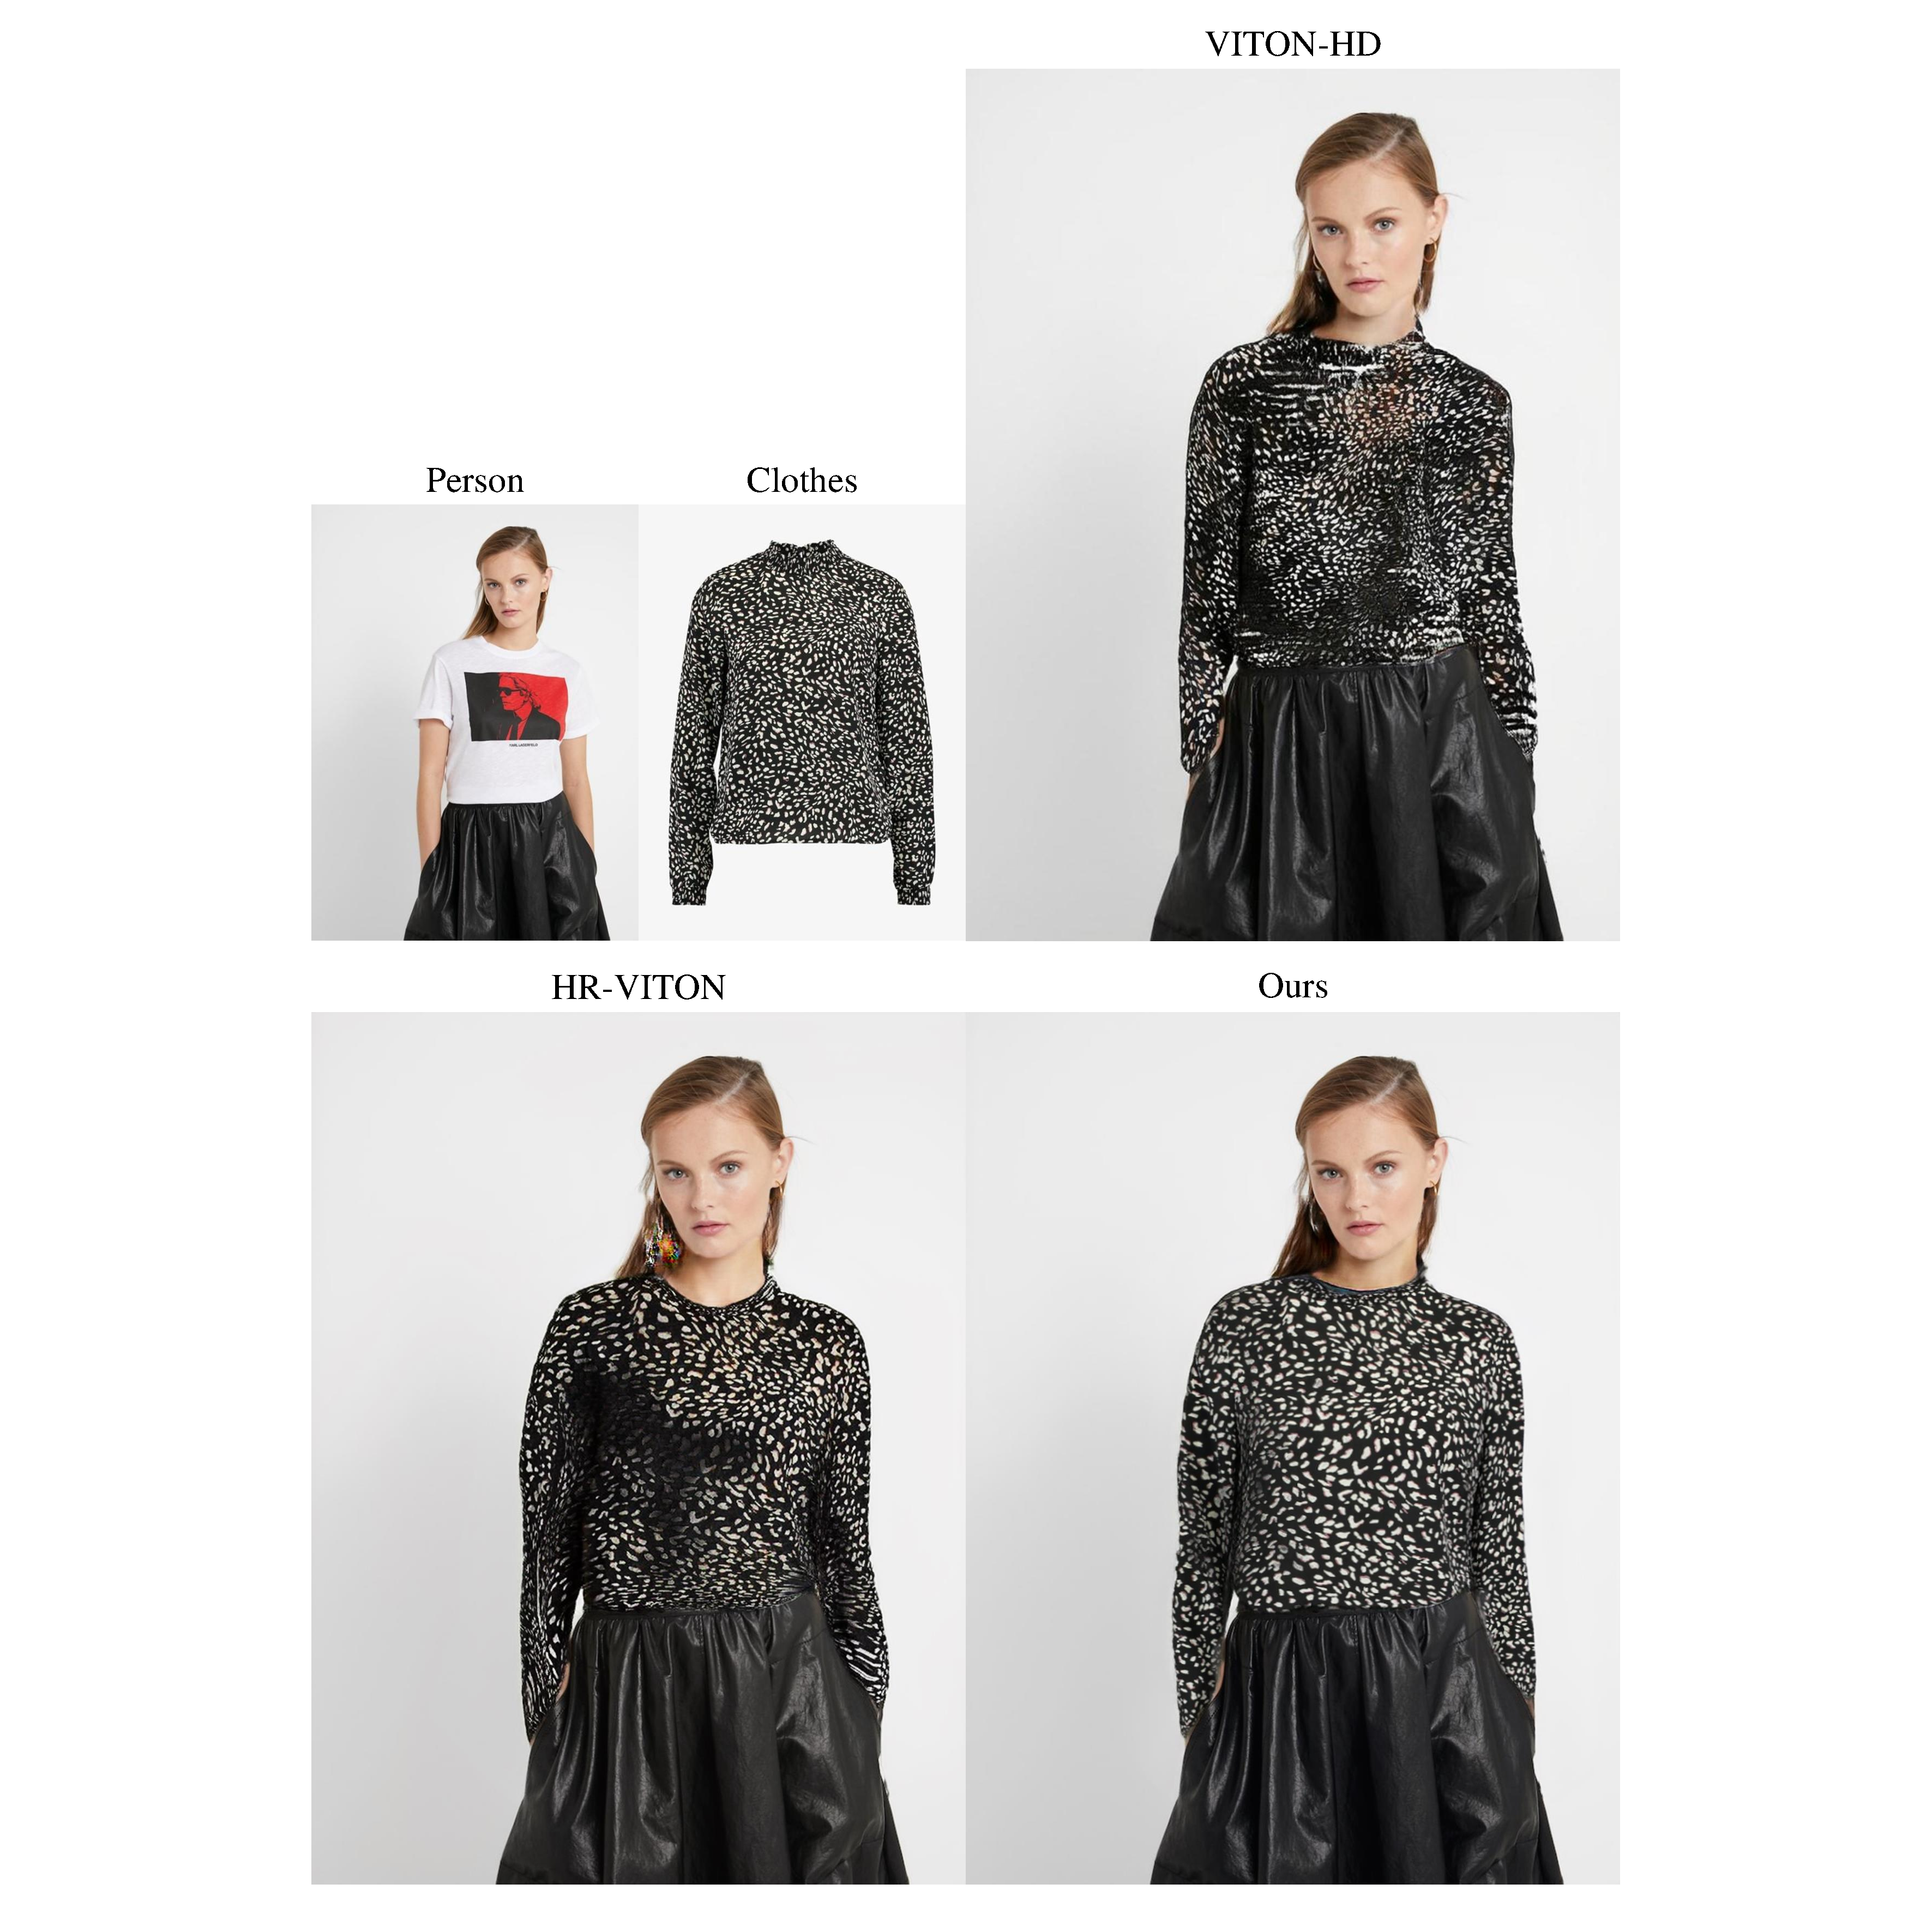
\includegraphics[width=0.85\textwidth]{fig_supp/fig_suppl_HD_2.pdf}
     \caption{Qualitative comparison between VITON-HD~\cite{choi2021viton}, HR-VITON~\cite{lee2022hrviton}, and ours. We recommend to look into the arm.
     }
     \label{fig_supp_longsleeve_HR_1}
\end{figure*}

\begin{figure*}[t!]
    \centering
     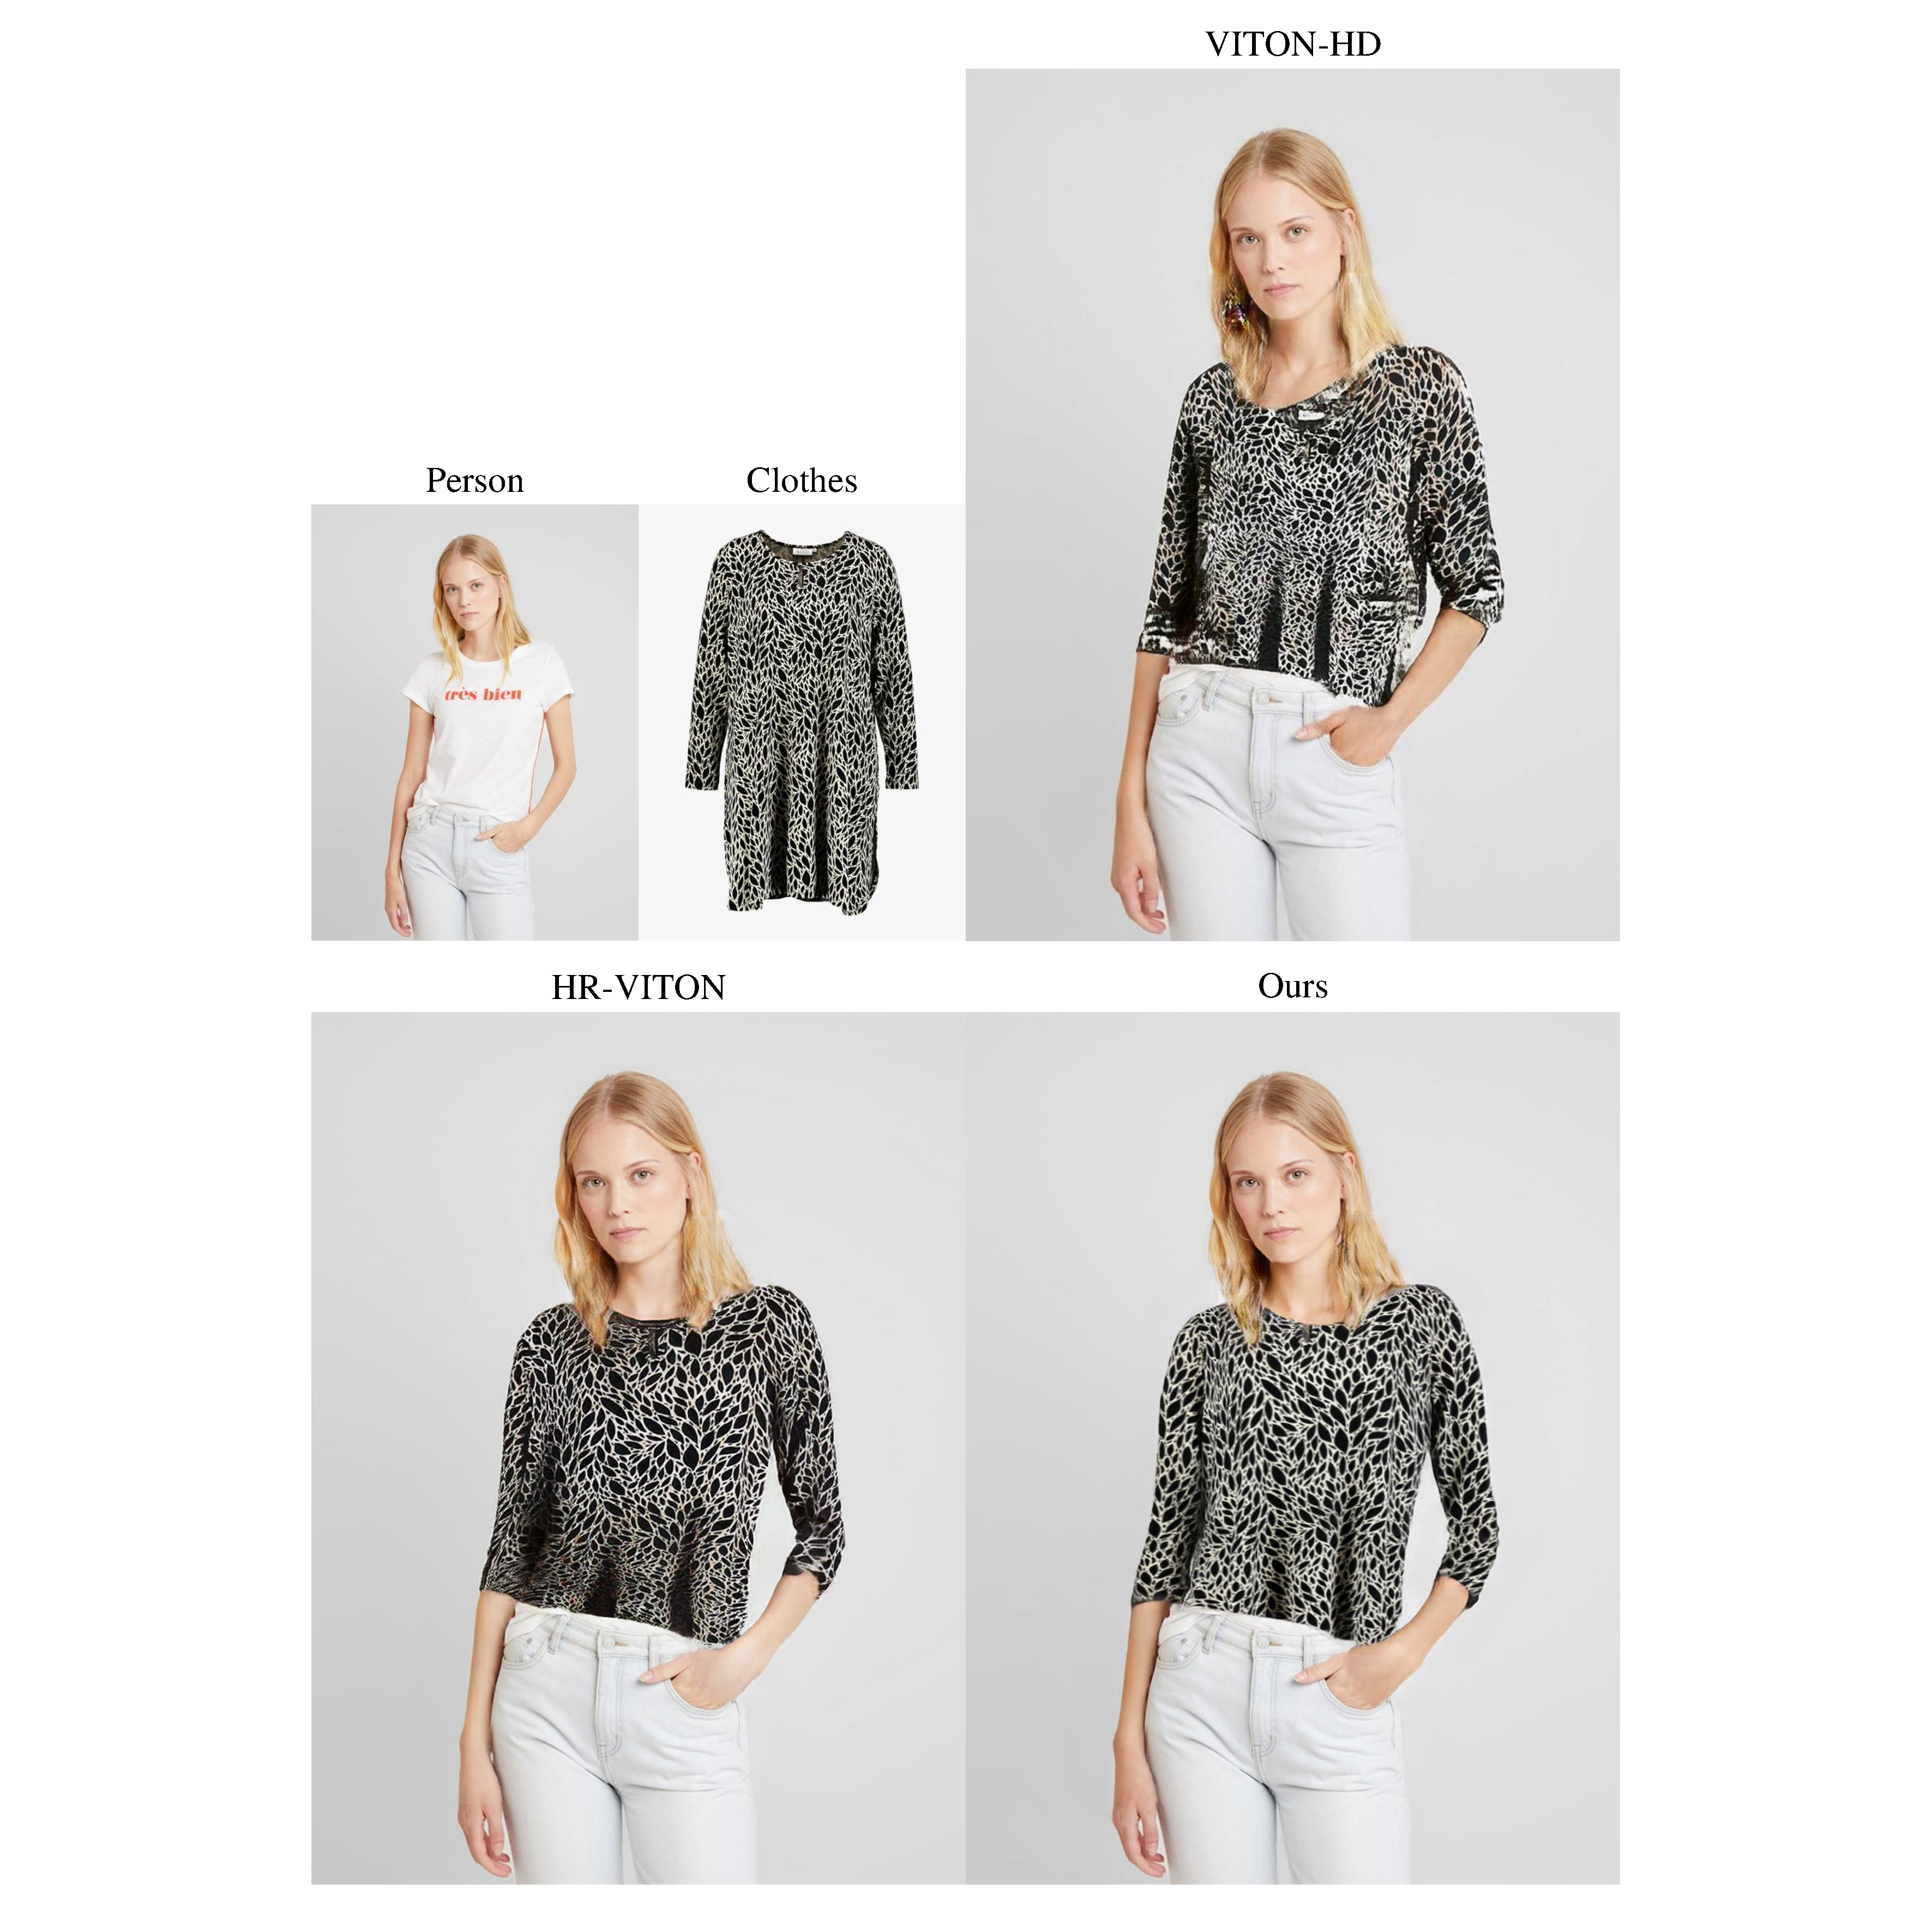
\includegraphics[width=0.85\textwidth]{fig_supp/fig_suppl_HD_1.pdf}
     \caption{Qualitative comparison between VITON-HD~\cite{choi2021viton}, HR-VITON~\cite{lee2022hrviton}, and ours. We recommend to look into the arm.
     }
     \label{fig_supp_longsleeve_HR_2}
\end{figure*}

\begin{figure*}[t!]
    \centering
     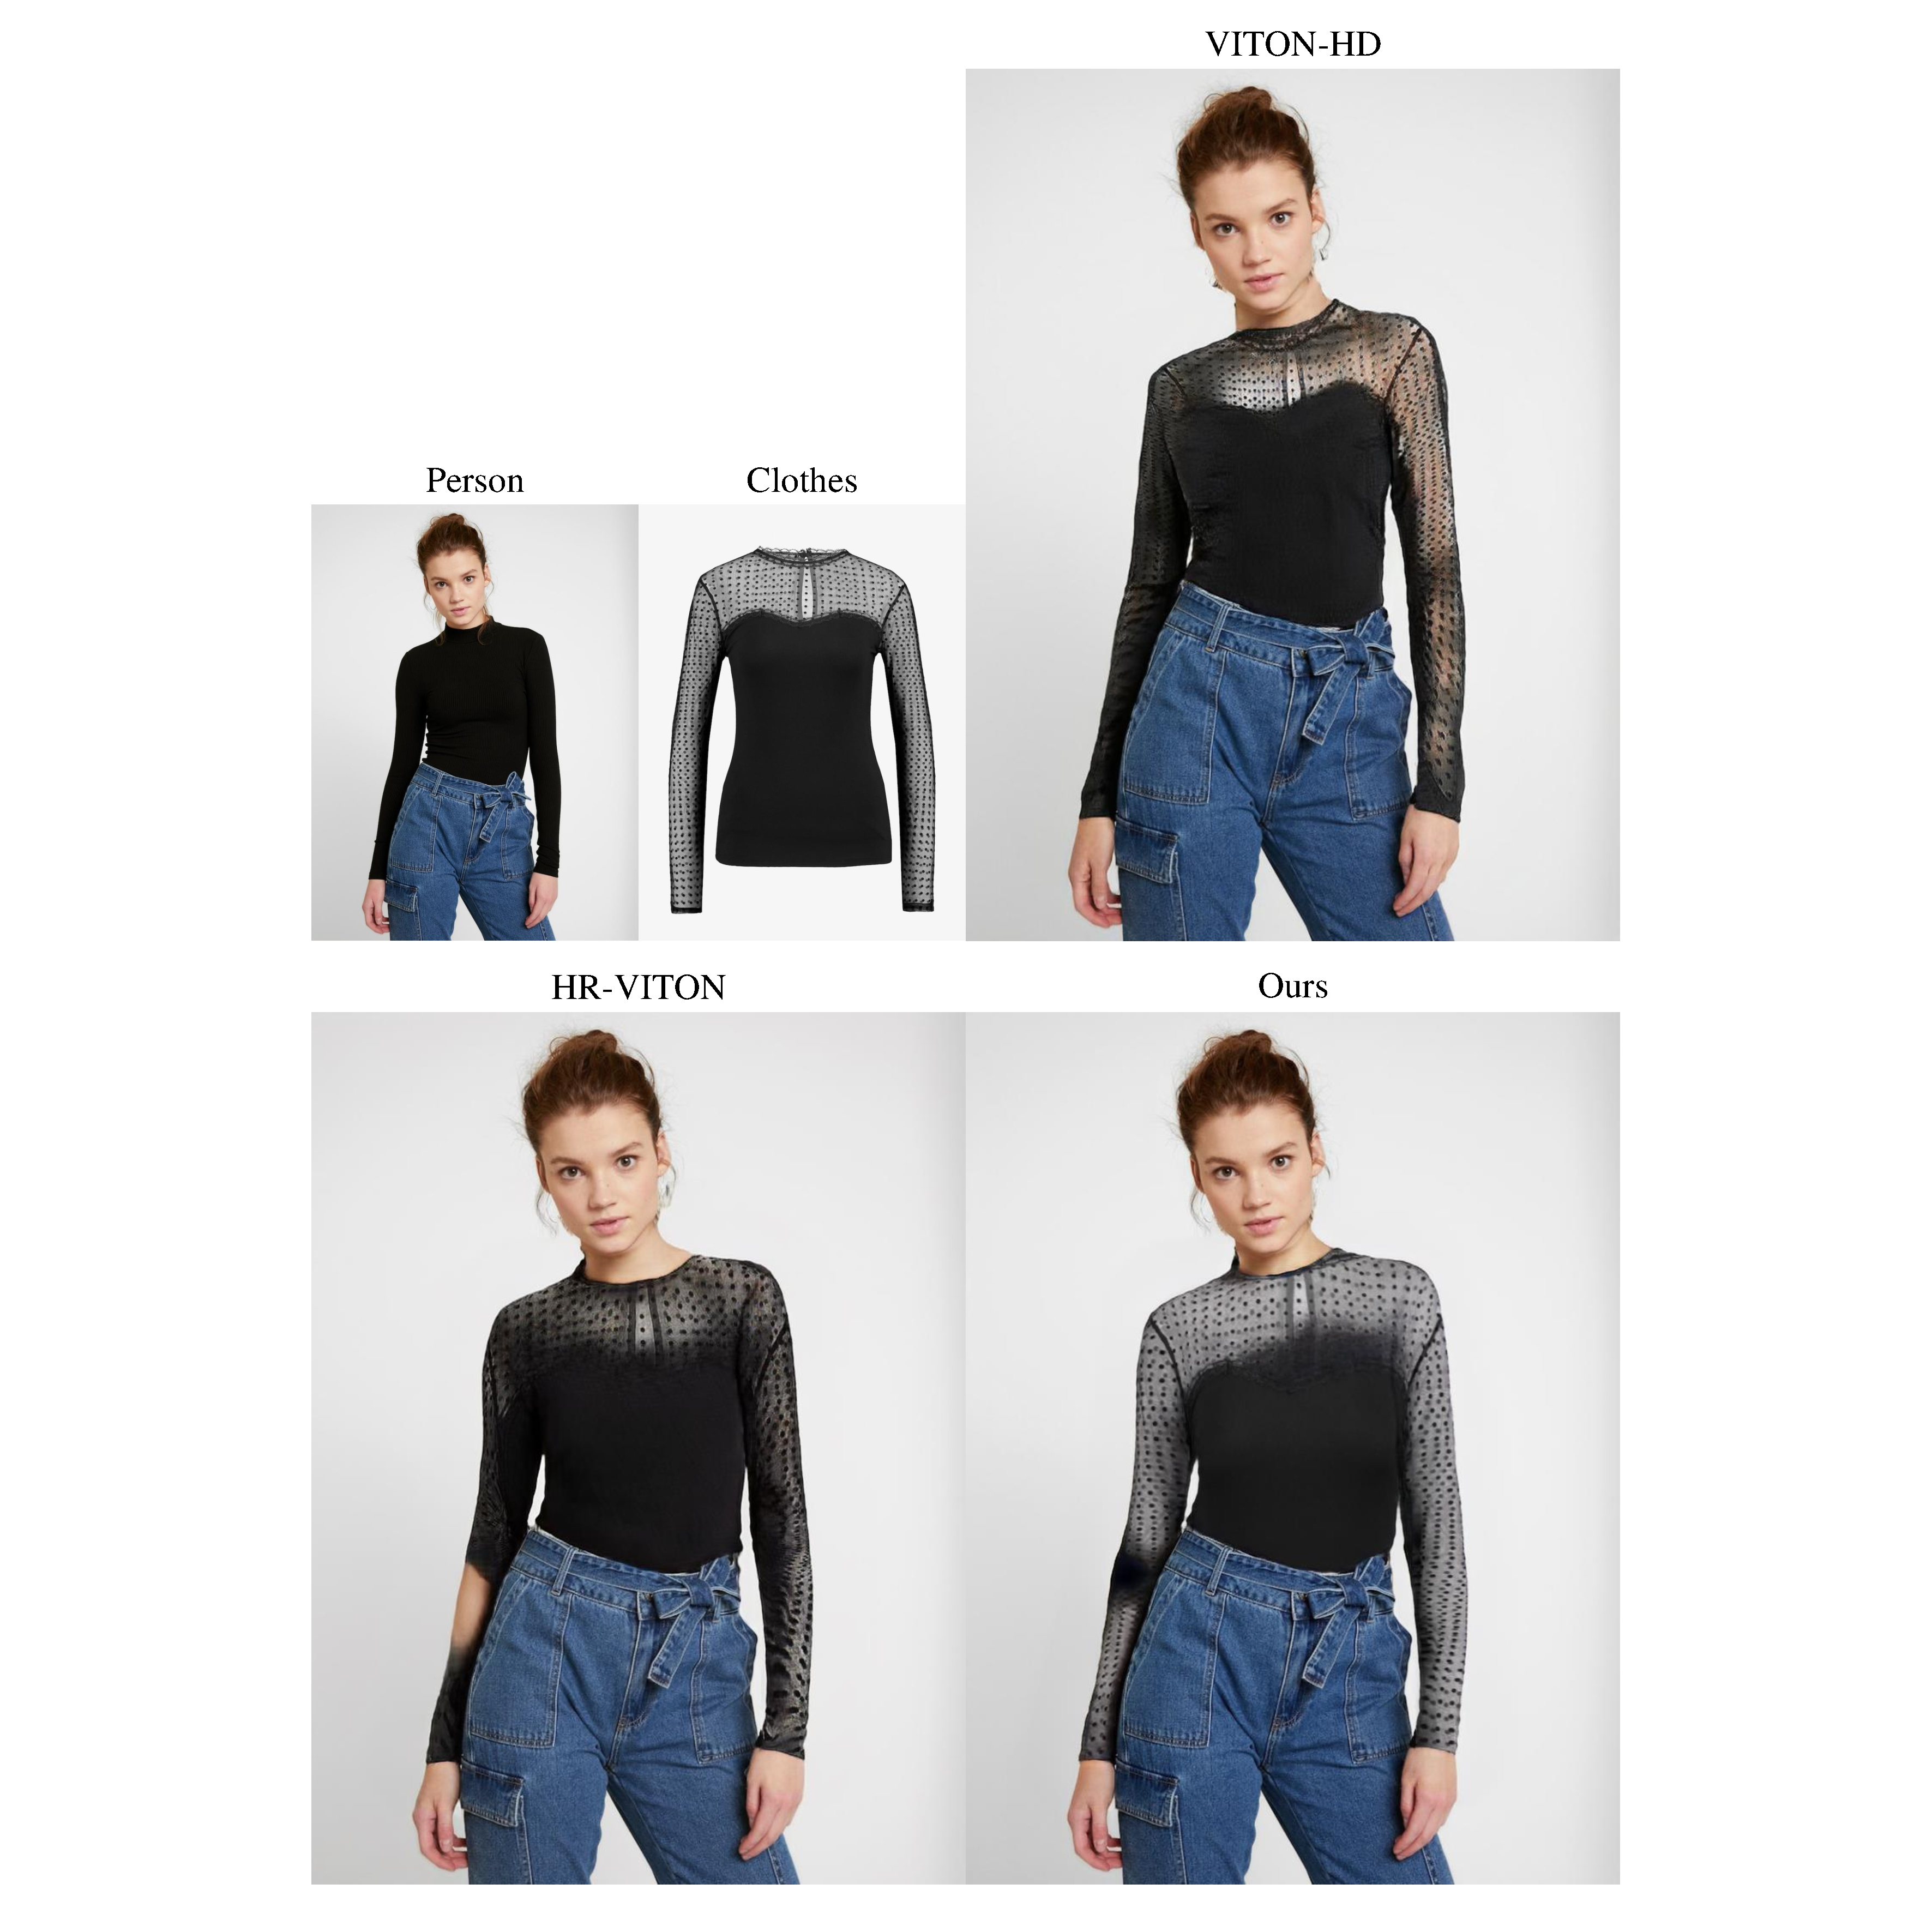
\includegraphics[width=0.85\textwidth]{fig_supp/fig_suppl_HD_0.pdf}
     \caption{Qualitative comparison between VITON-HD~\cite{choi2021viton}, HR-VITON~\cite{lee2022hrviton}, and ours. We recommend to look into the arm.
     }
     \label{fig_supp_longsleeve_HR_3}
\end{figure*}

\begin{figure*}[t!]
    \centering
     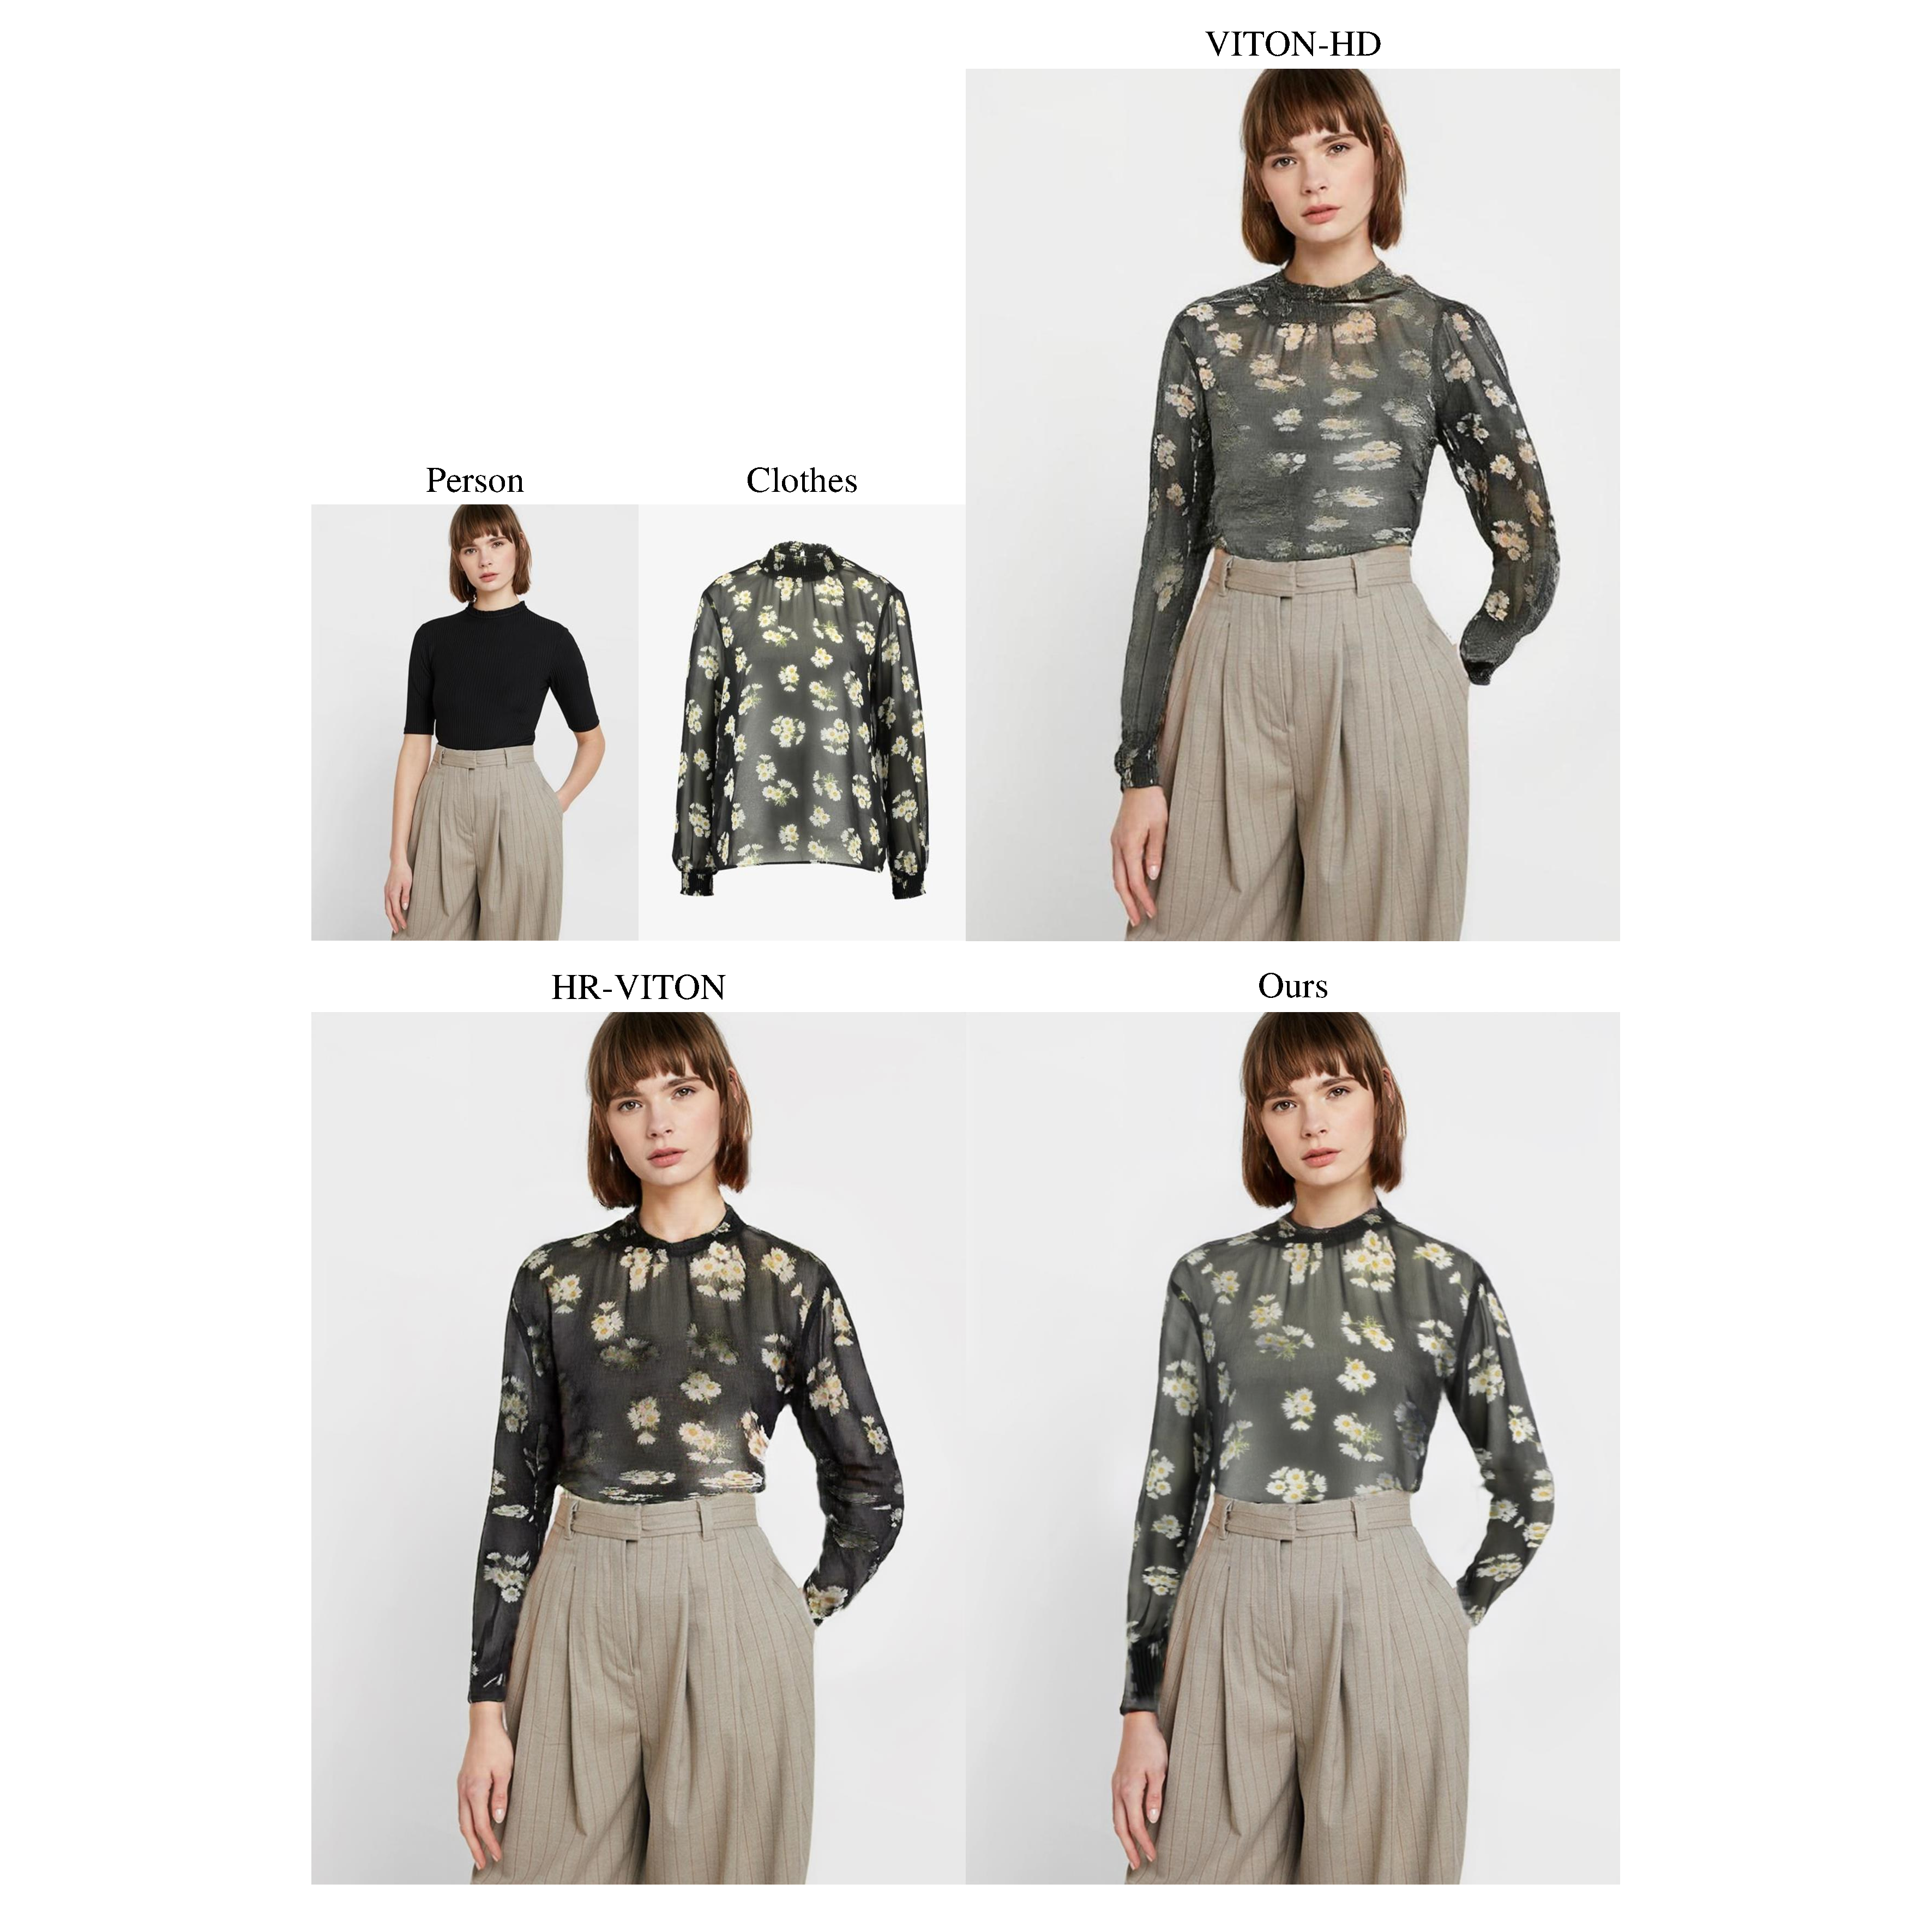
\includegraphics[width=0.85\textwidth]{fig_supp/fig_suppl_HD_4.pdf}
     \caption{Qualitative comparison between VITON-HD~\cite{choi2021viton}, HR-VITON~\cite{lee2022hrviton}, and ours. We recommend to look into the arm.
     }
     \label{fig_supp_longsleeve_HR_4}
\end{figure*}

\begin{figure*}[t!]
    \centering
     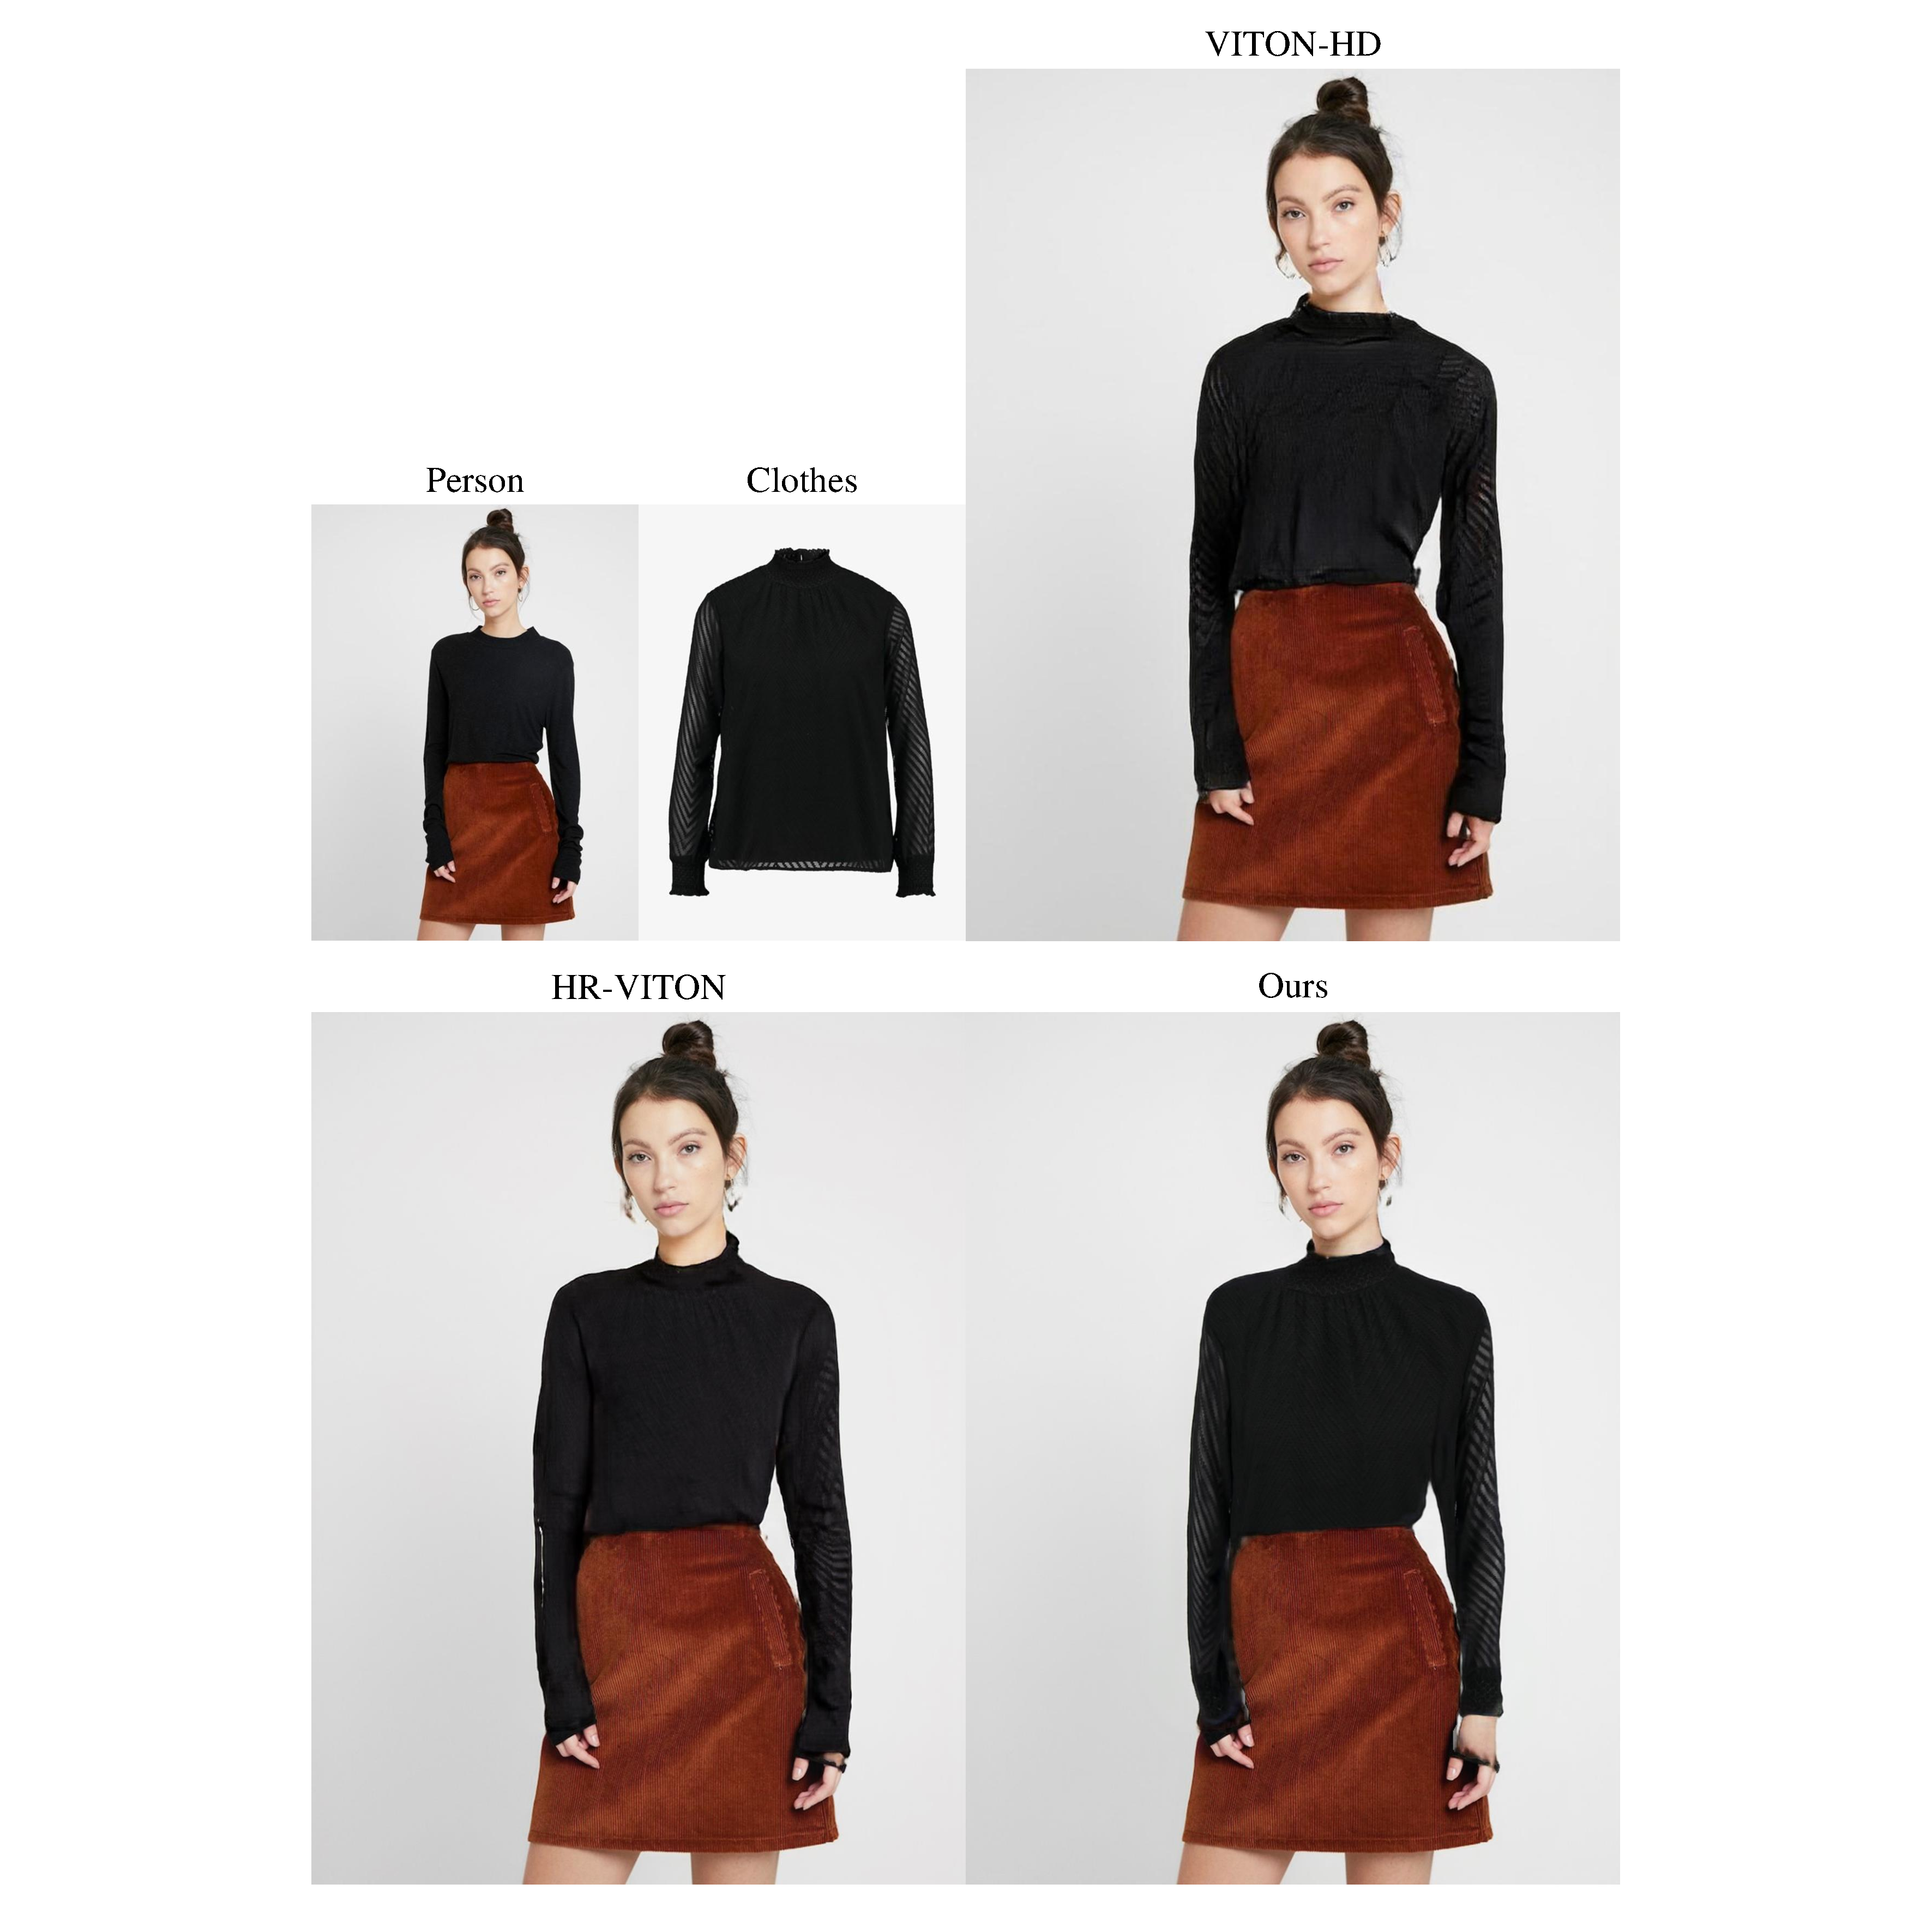
\includegraphics[width=0.85\textwidth]{fig_supp/fig_suppl_HD_5.pdf}
     \caption{Qualitative comparison between VITON-HD~\cite{choi2021viton}, HR-VITON~\cite{lee2022hrviton}, and ours. We recommend to look into the arm.
     }
     \label{fig_supp_longsleeve_HR_5}
\end{figure*}

\begin{figure*}[t!]
    \centering
     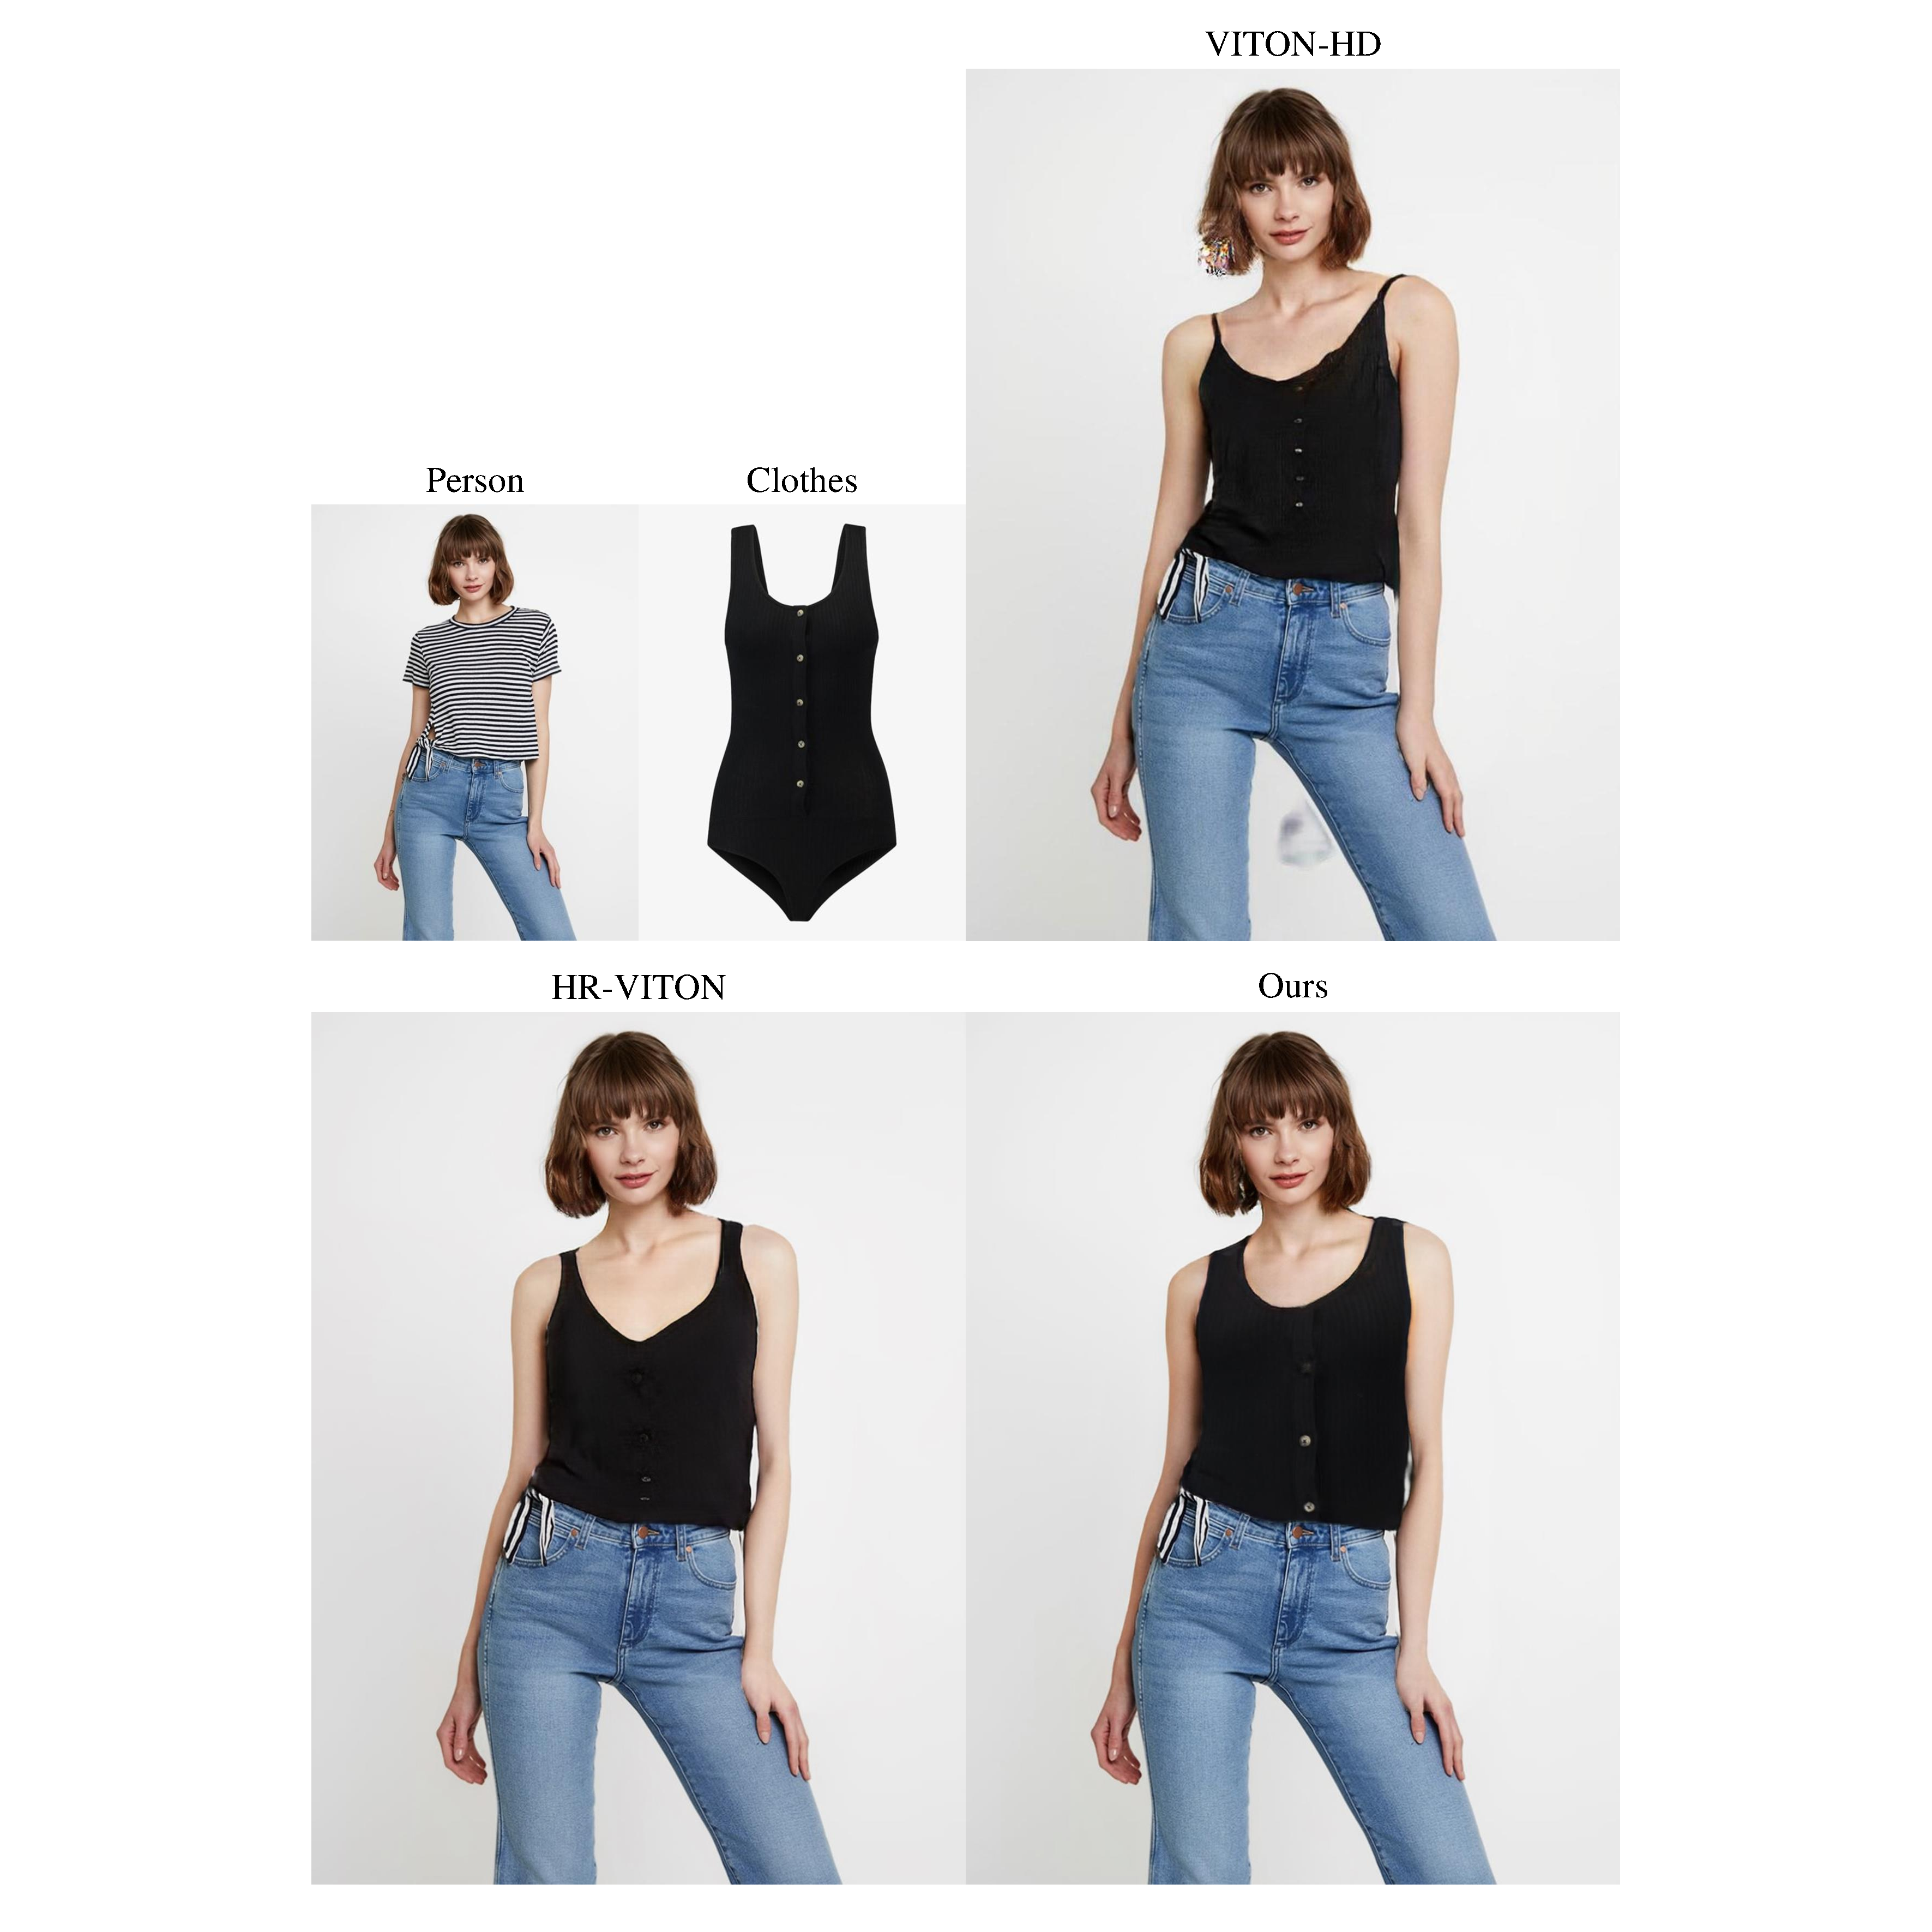
\includegraphics[width=0.85\textwidth]{fig_supp/fig_suppl_HD_6.pdf}
     \caption{Qualitative comparison between VITON-HD~\cite{choi2021viton}, HR-VITON~\cite{lee2022hrviton}, and ours. We recommend to look into the waist.
     }
     \label{fig_supp_tucked_in_HR_6}
\end{figure*}

\begin{figure*}[t!]
    \centering
     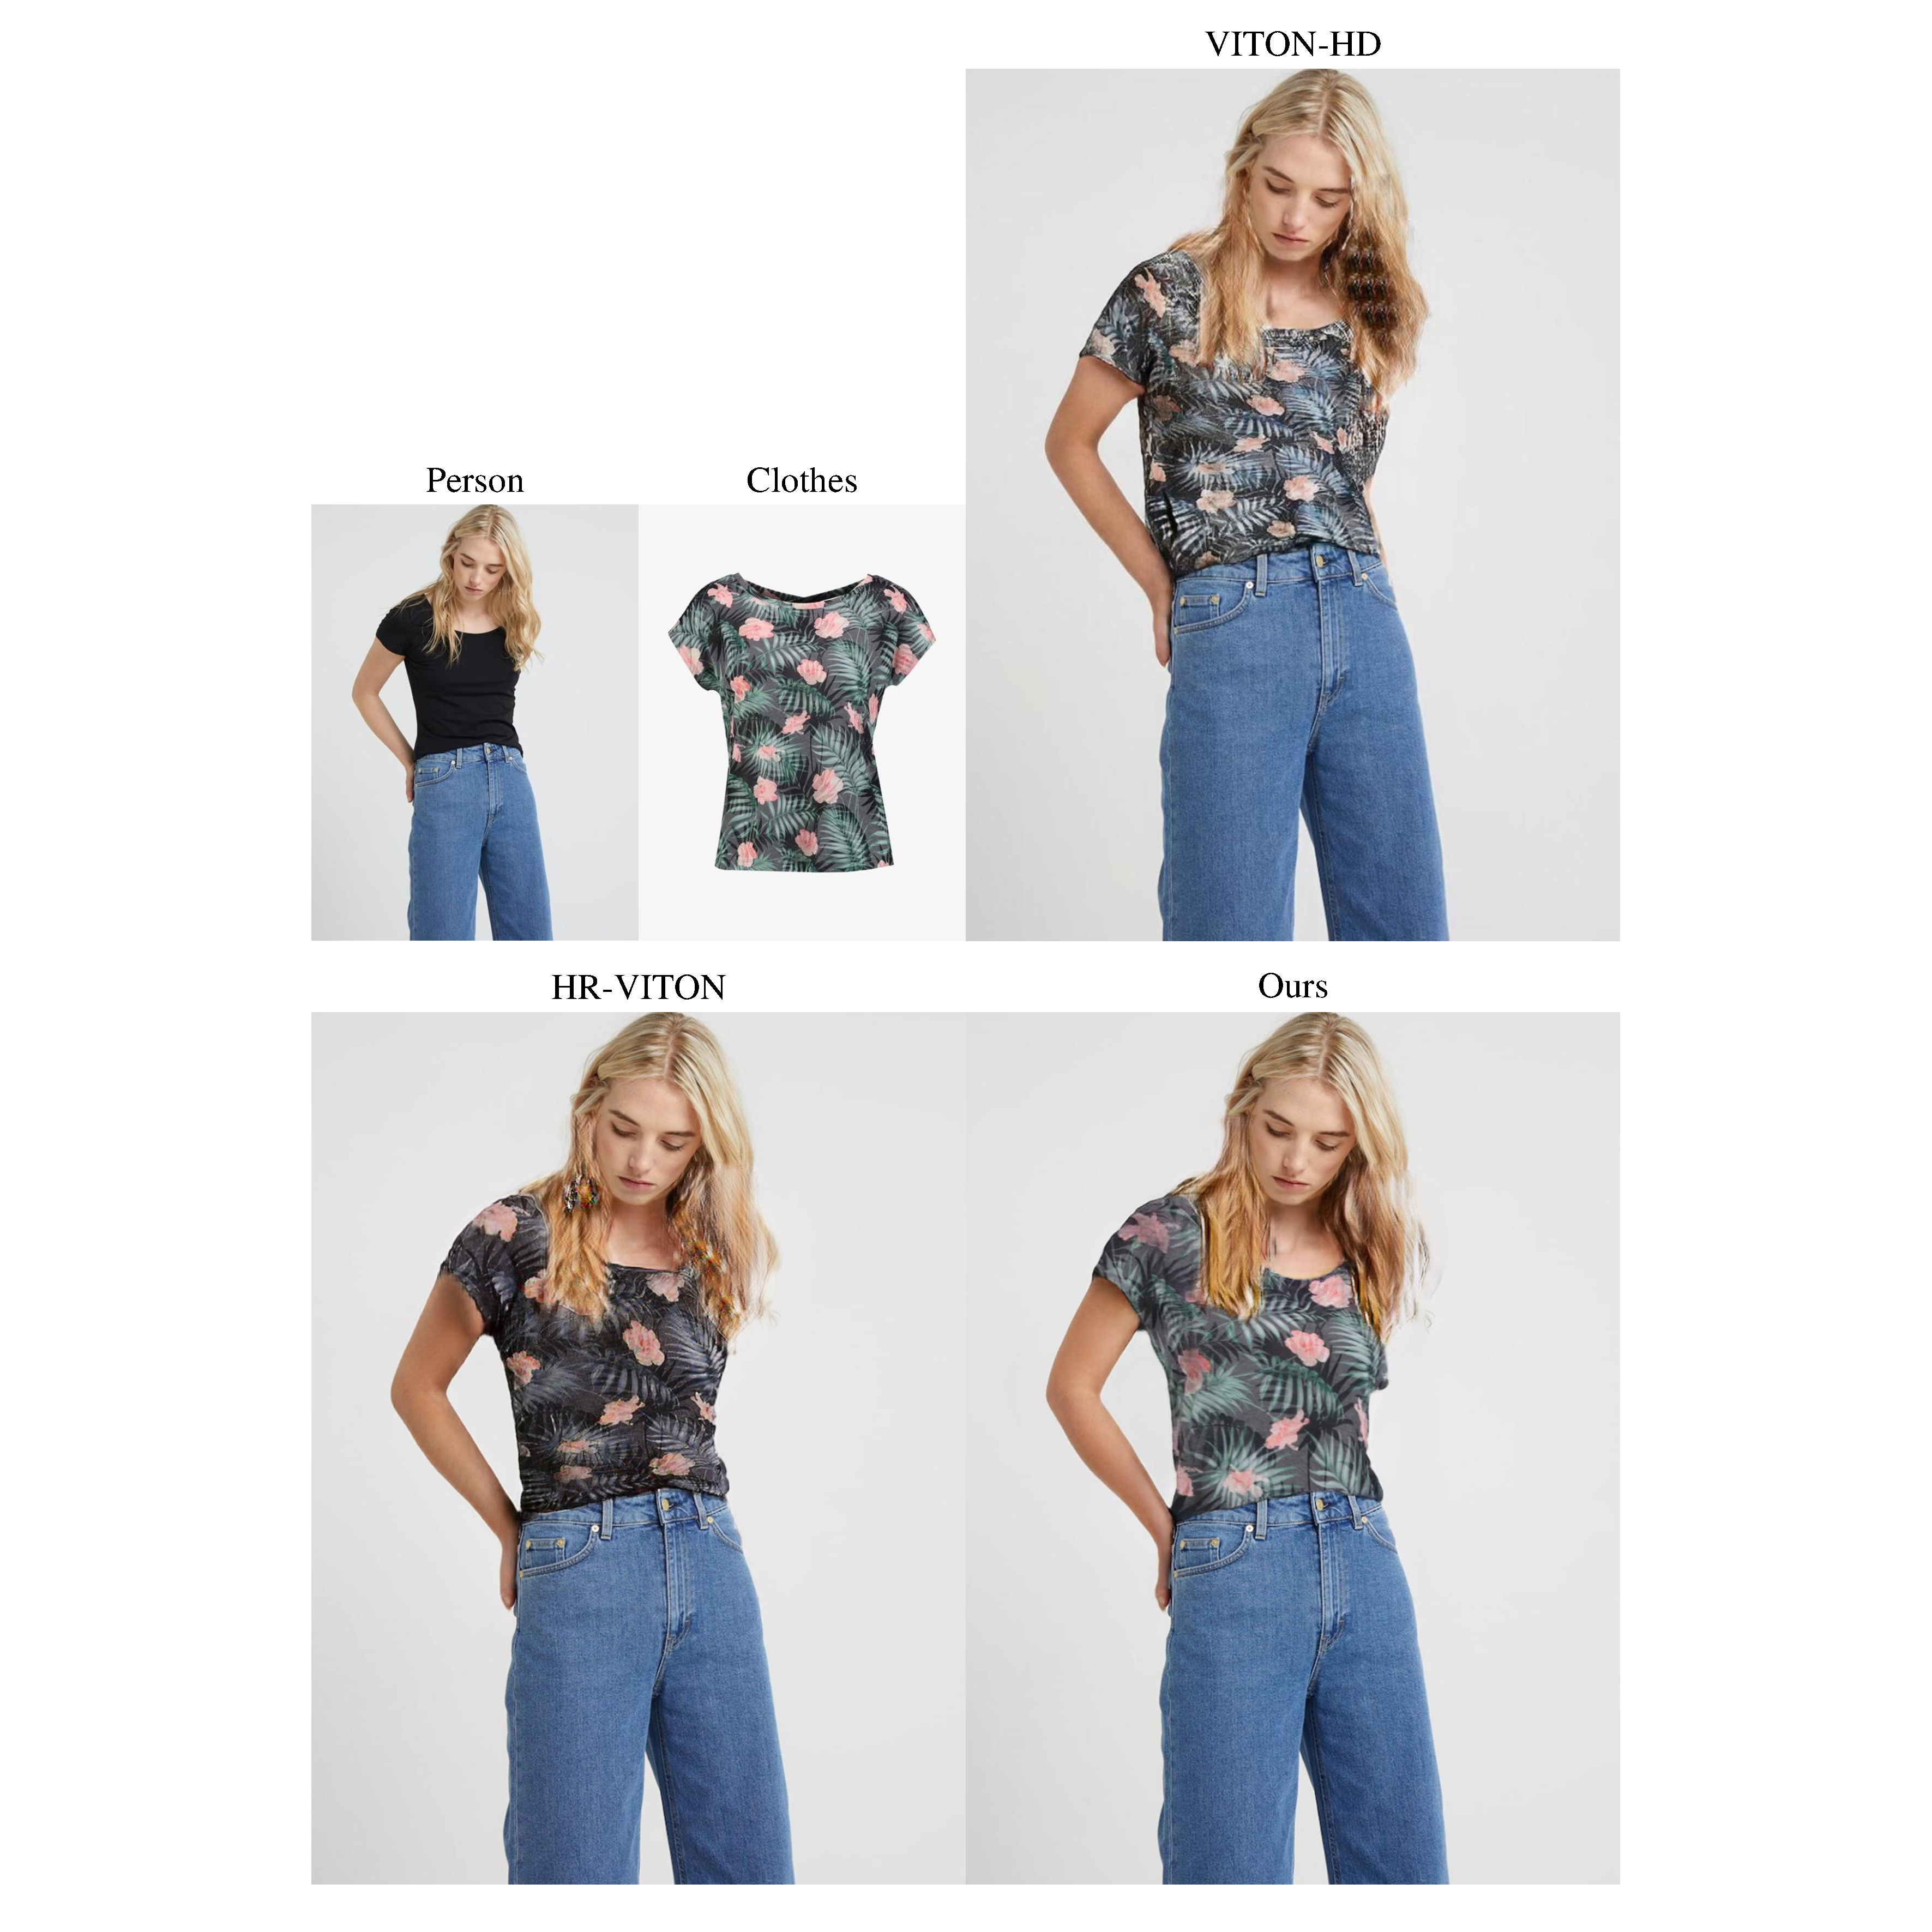
\includegraphics[width=0.85\textwidth]{fig_supp/fig_suppl_HD_7.pdf}
     \caption{Qualitative comparison between VITON-HD~\cite{choi2021viton}, HR-VITON~\cite{lee2022hrviton}, and ours. We recommend to look into the waist.
     }
     \label{fig_supp_tucked_in_HR_7}
\end{figure*}

\begin{figure*}[t!]
    \centering
     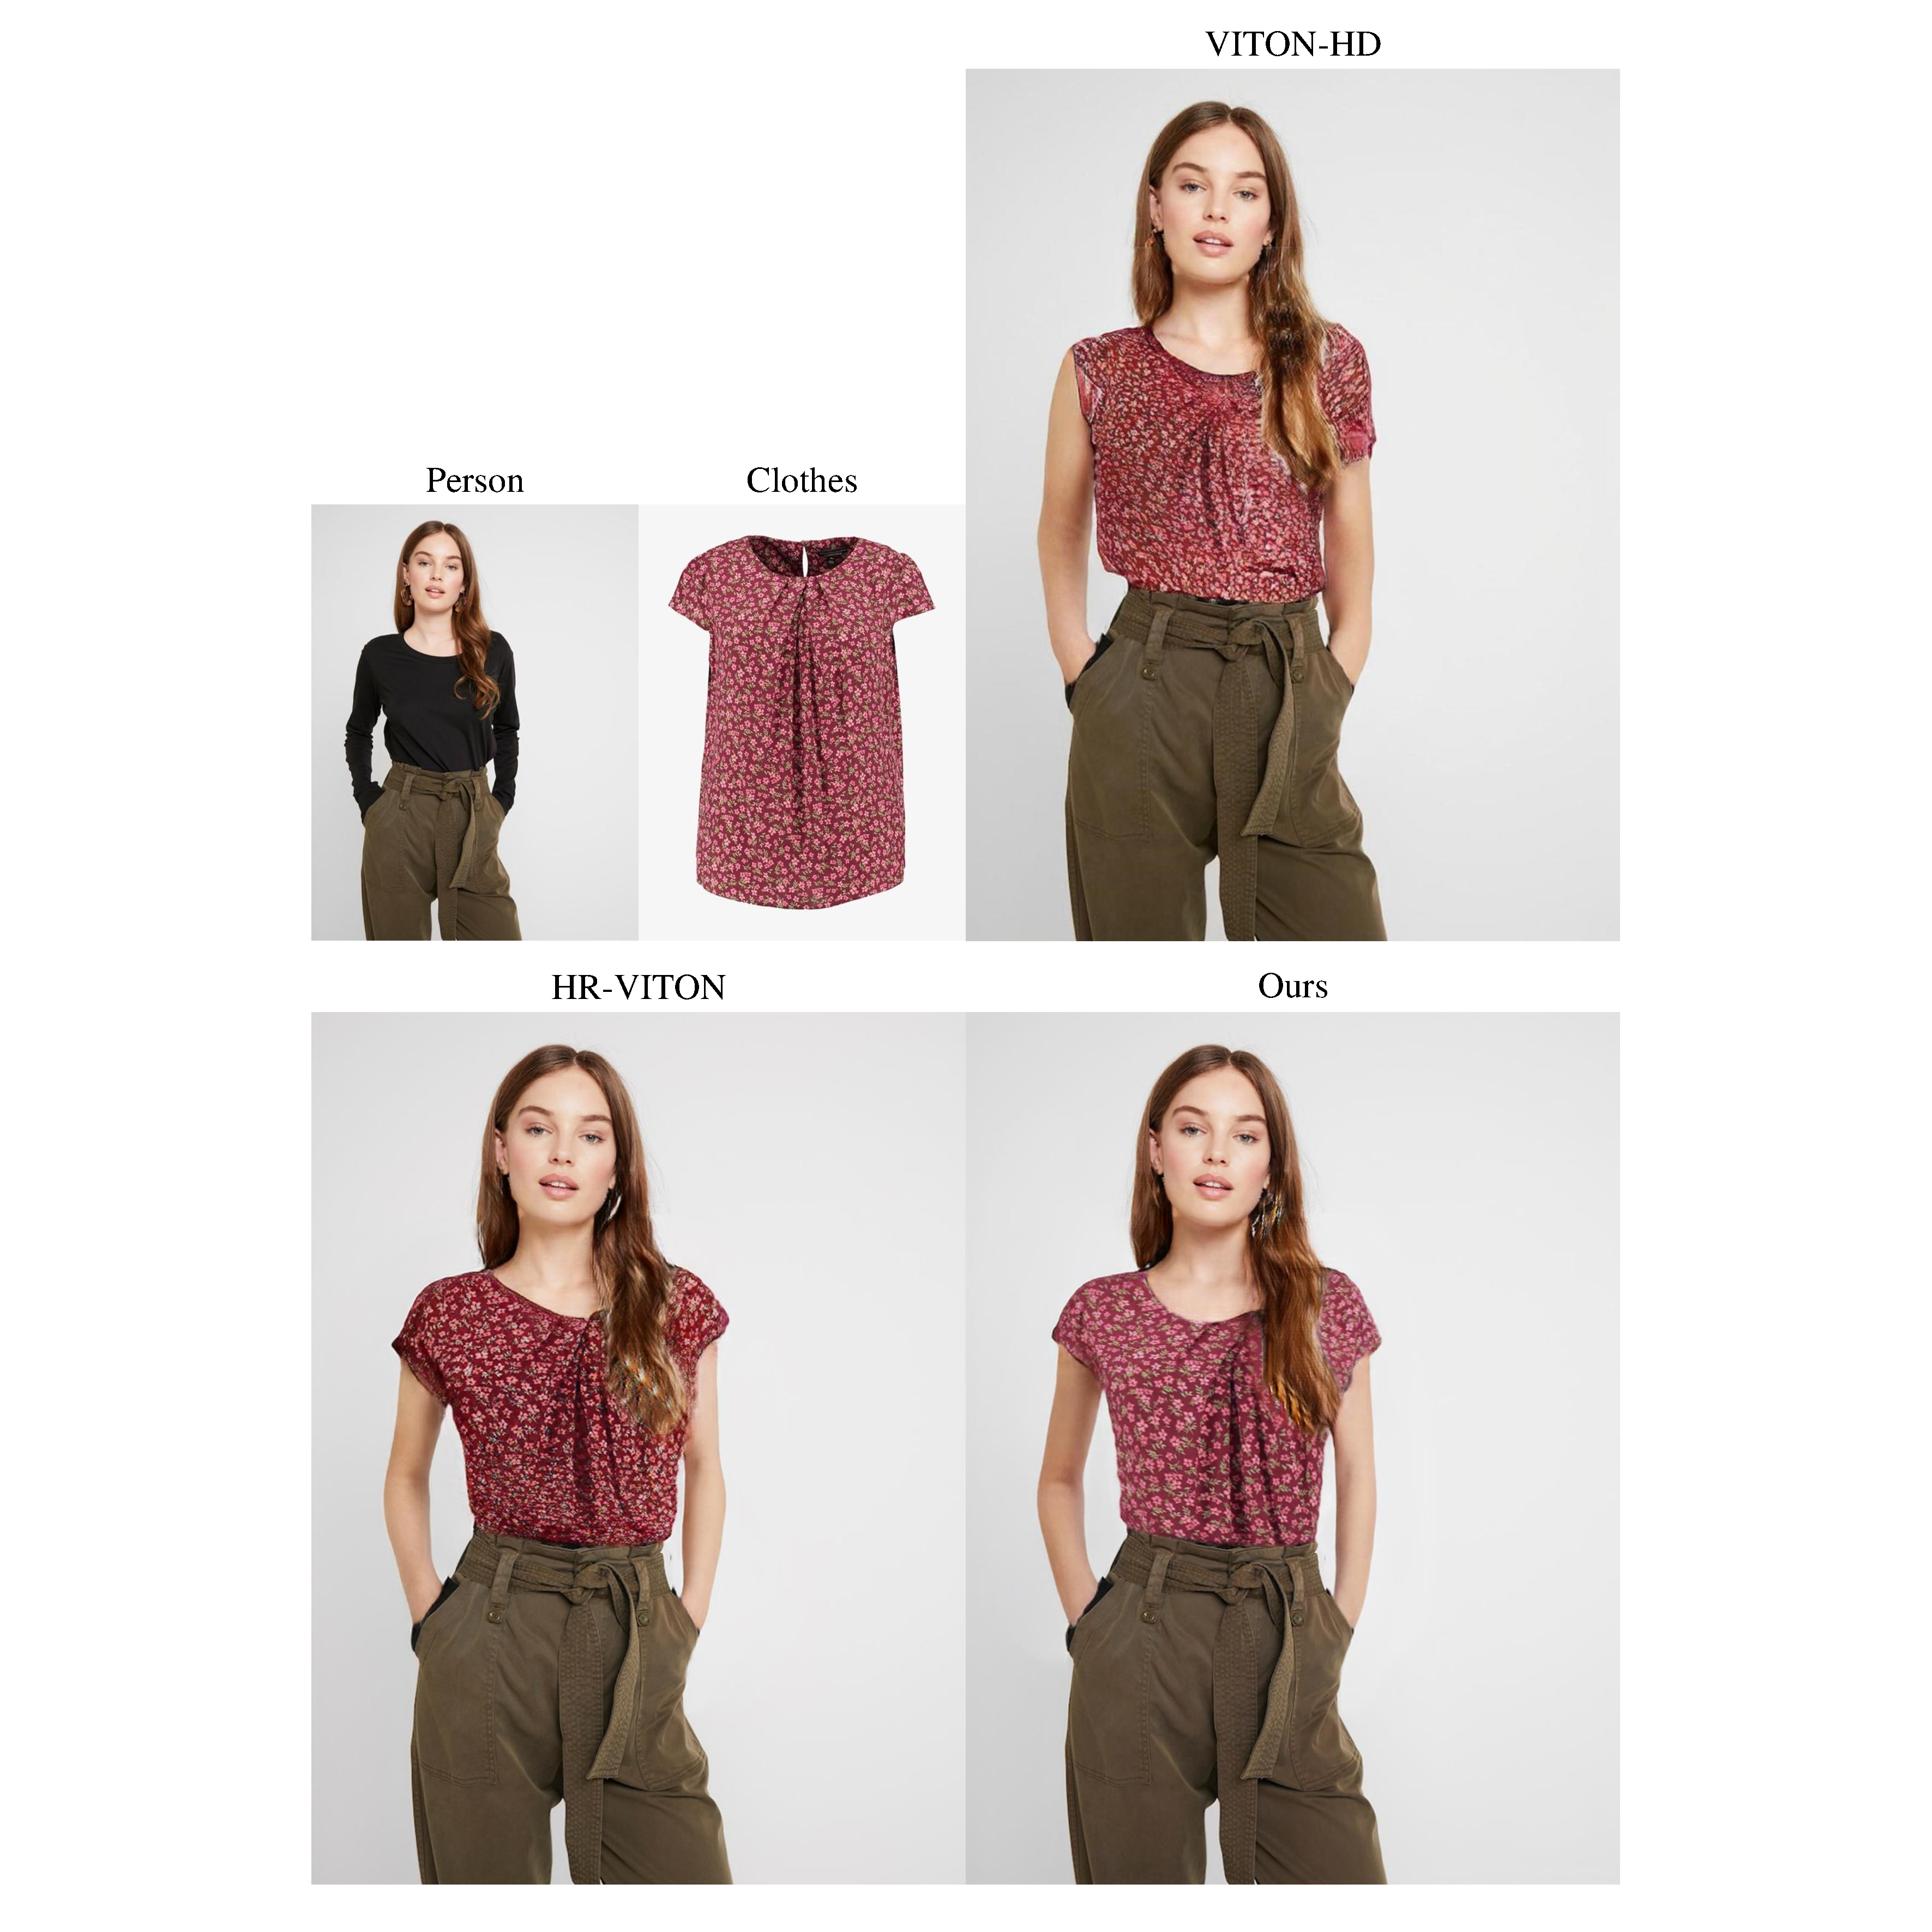
\includegraphics[width=0.85\textwidth]{fig_supp/fig_suppl_HD_8.pdf}
     \caption{Qualitative comparison between VITON-HD~\cite{choi2021viton}, HR-VITON~\cite{lee2022hrviton}, and ours. We recommend to look into the waist.
     }
     \label{fig_supp_tucked_in_HR_8}
\end{figure*}

\begin{figure*}[t!]
    \centering
     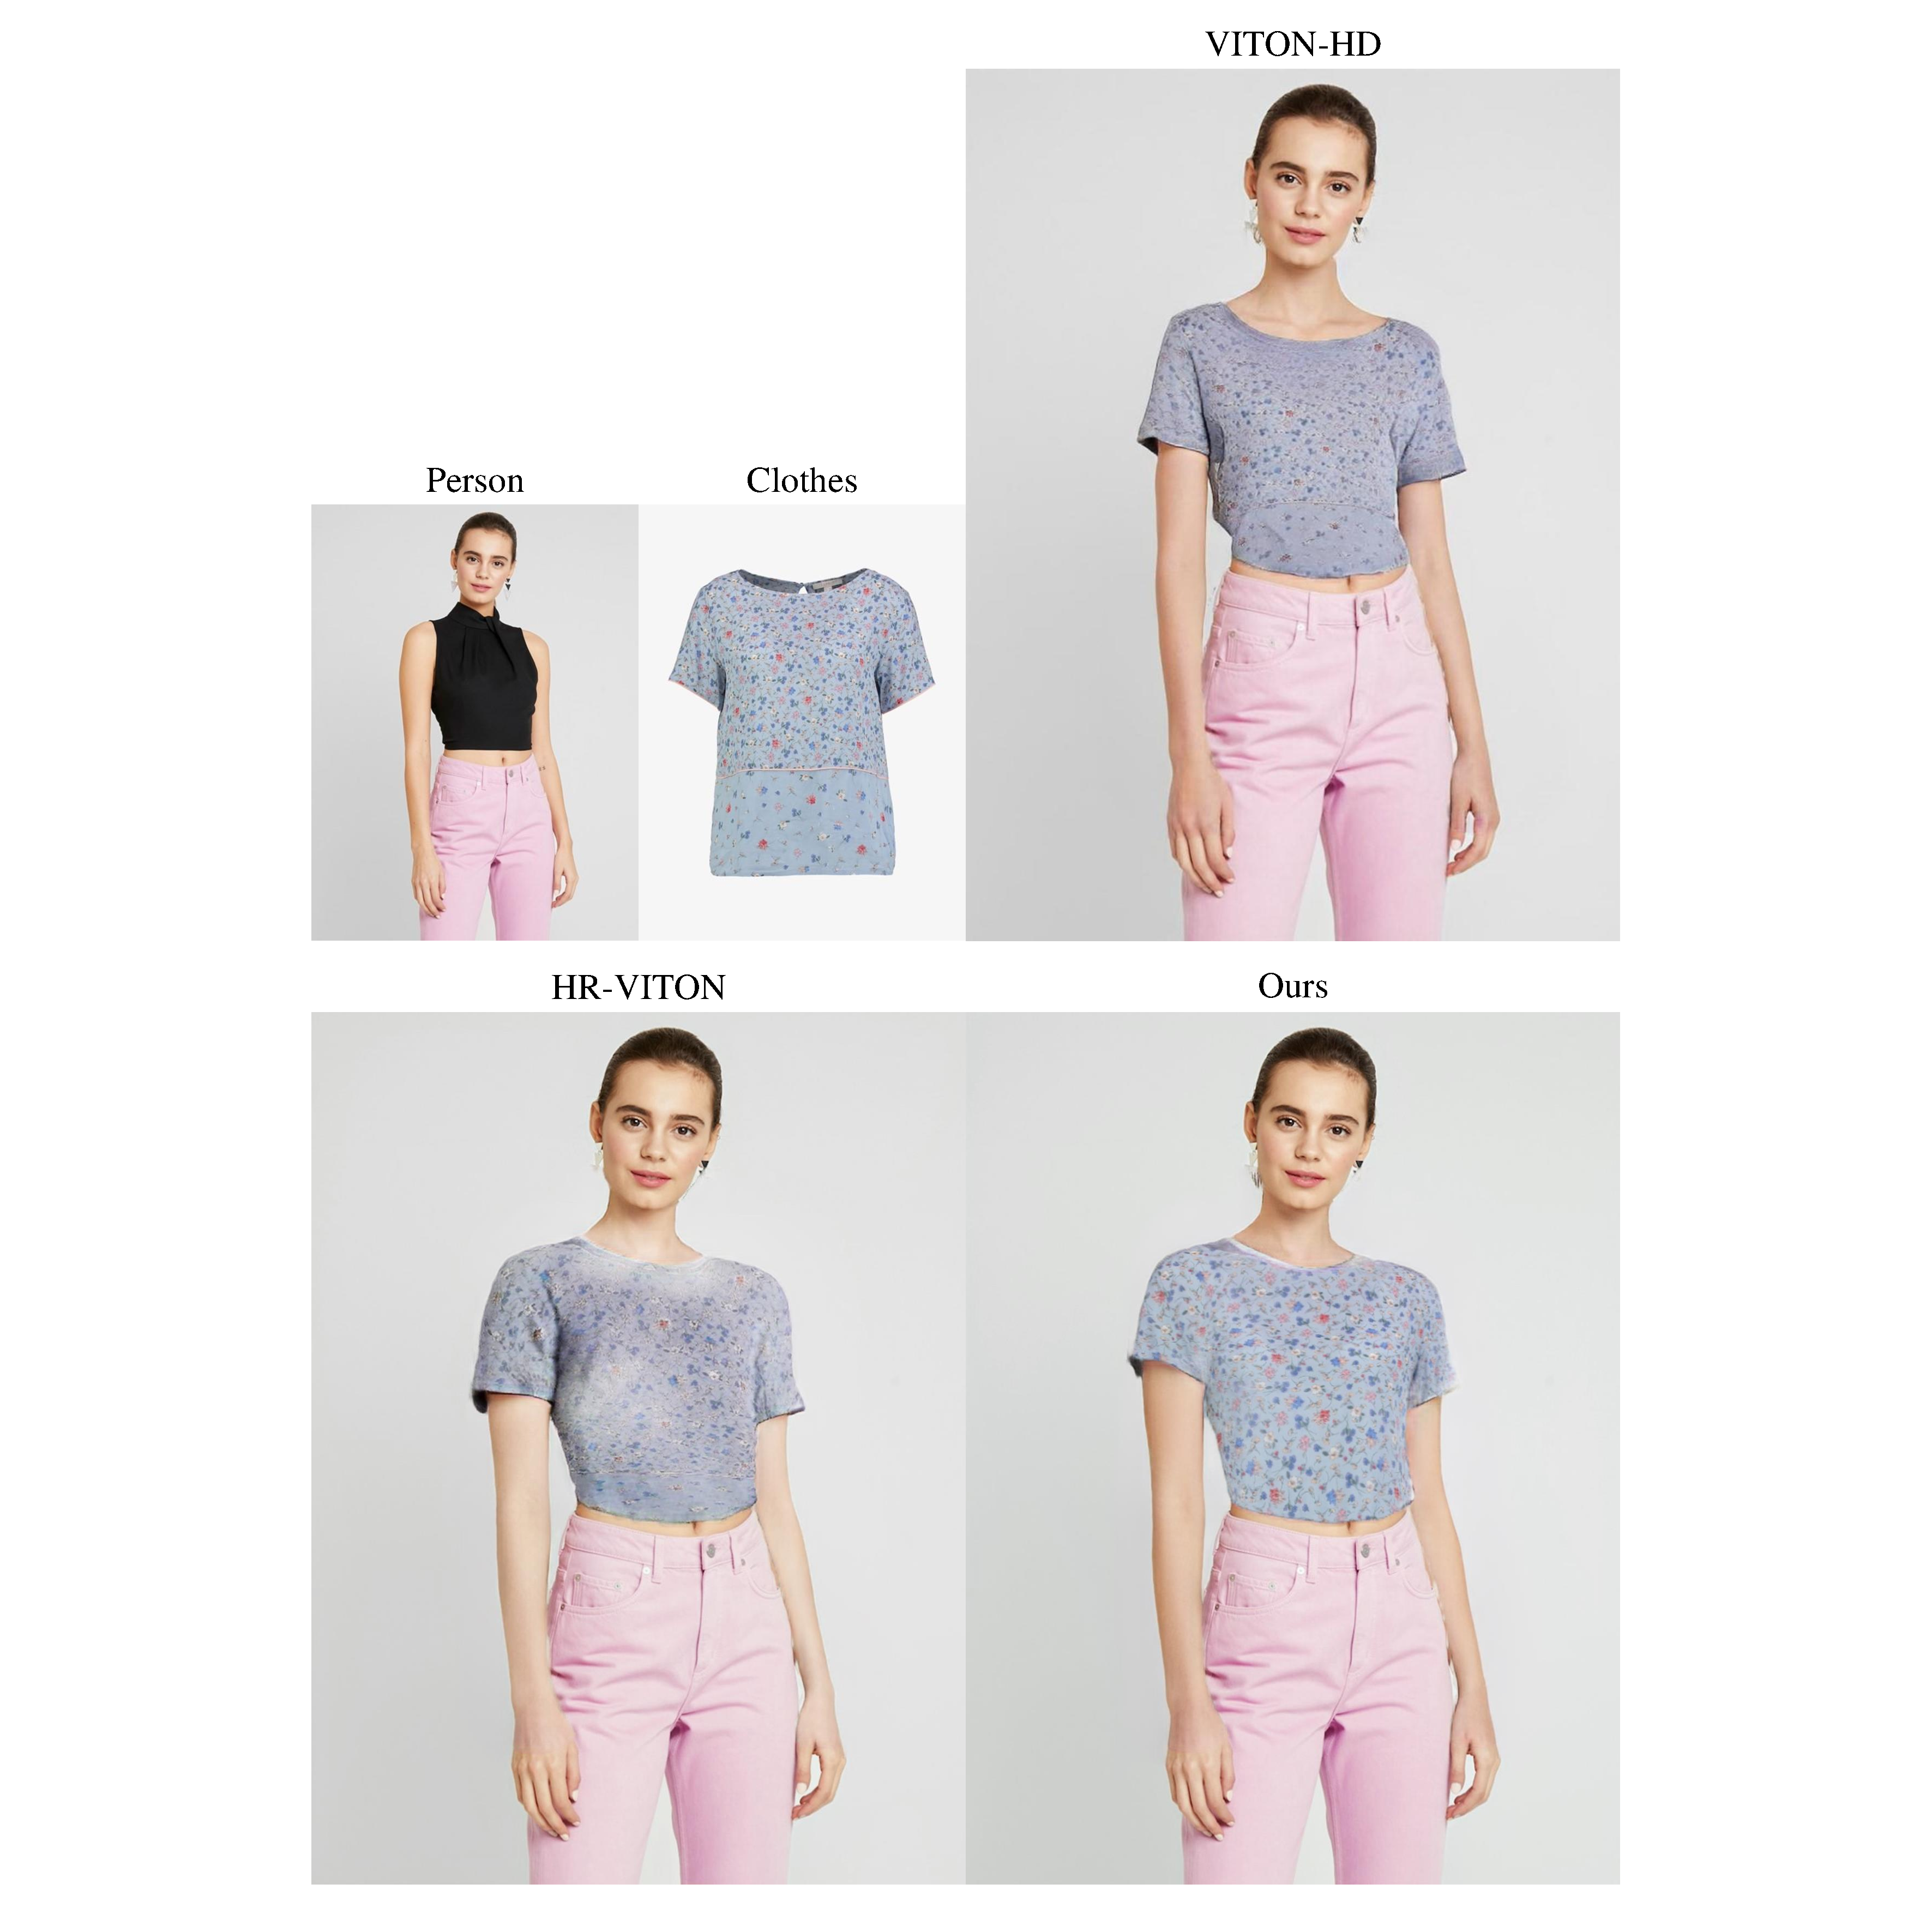
\includegraphics[width=0.85\textwidth]{fig_supp/fig_suppl_HD_9.pdf}
     \caption{Qualitative comparison between VITON-HD~\cite{choi2021viton}, HR-VITON~\cite{lee2022hrviton}, and ours. We recommend to look into the waist.
     }
     \label{fig_supp_tucked_in_HR_9}
\end{figure*}

\begin{figure*}[t!]
    \centering
     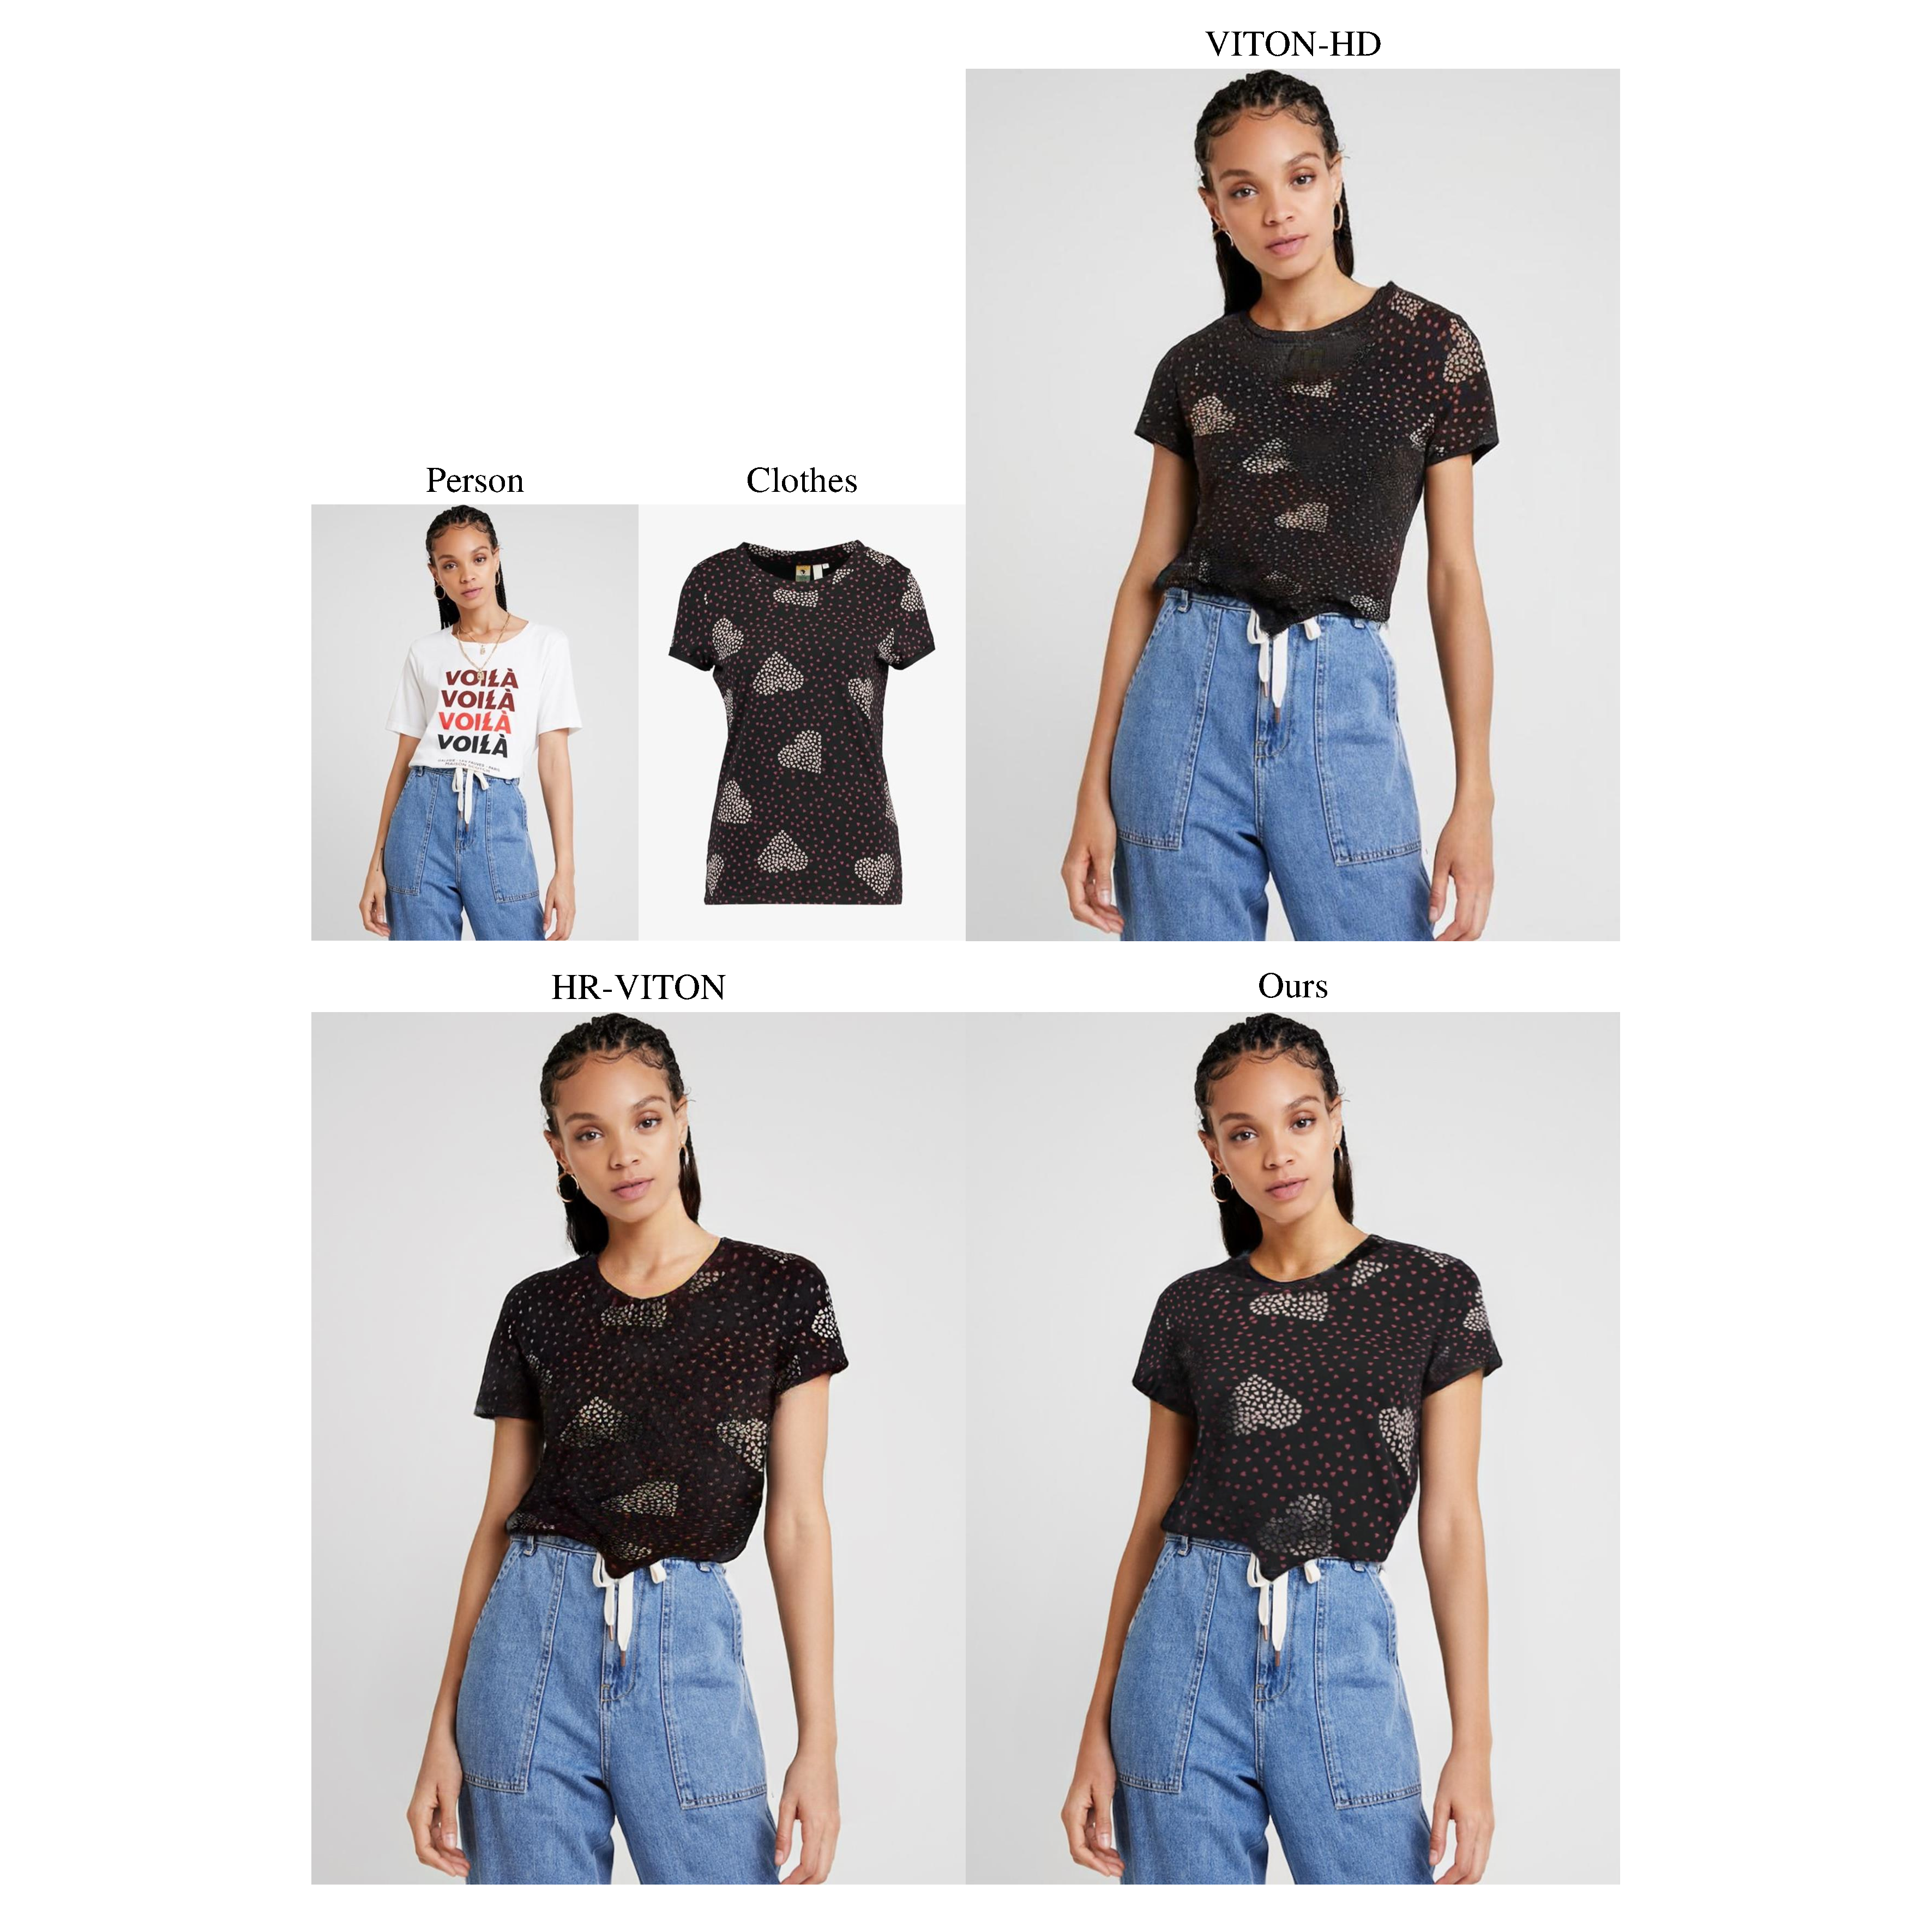
\includegraphics[width=0.85\textwidth]{fig_supp/fig_suppl_HD_10.pdf}
     \caption{Qualitative comparison between VITON-HD~\cite{choi2021viton}, HR-VITON~\cite{lee2022hrviton}, and ours. We recommend to look into the waist.
     }
     \label{fig_supp_tucked_in_HR_10}
\end{figure*}

\begin{figure*}[t!]
    \centering
     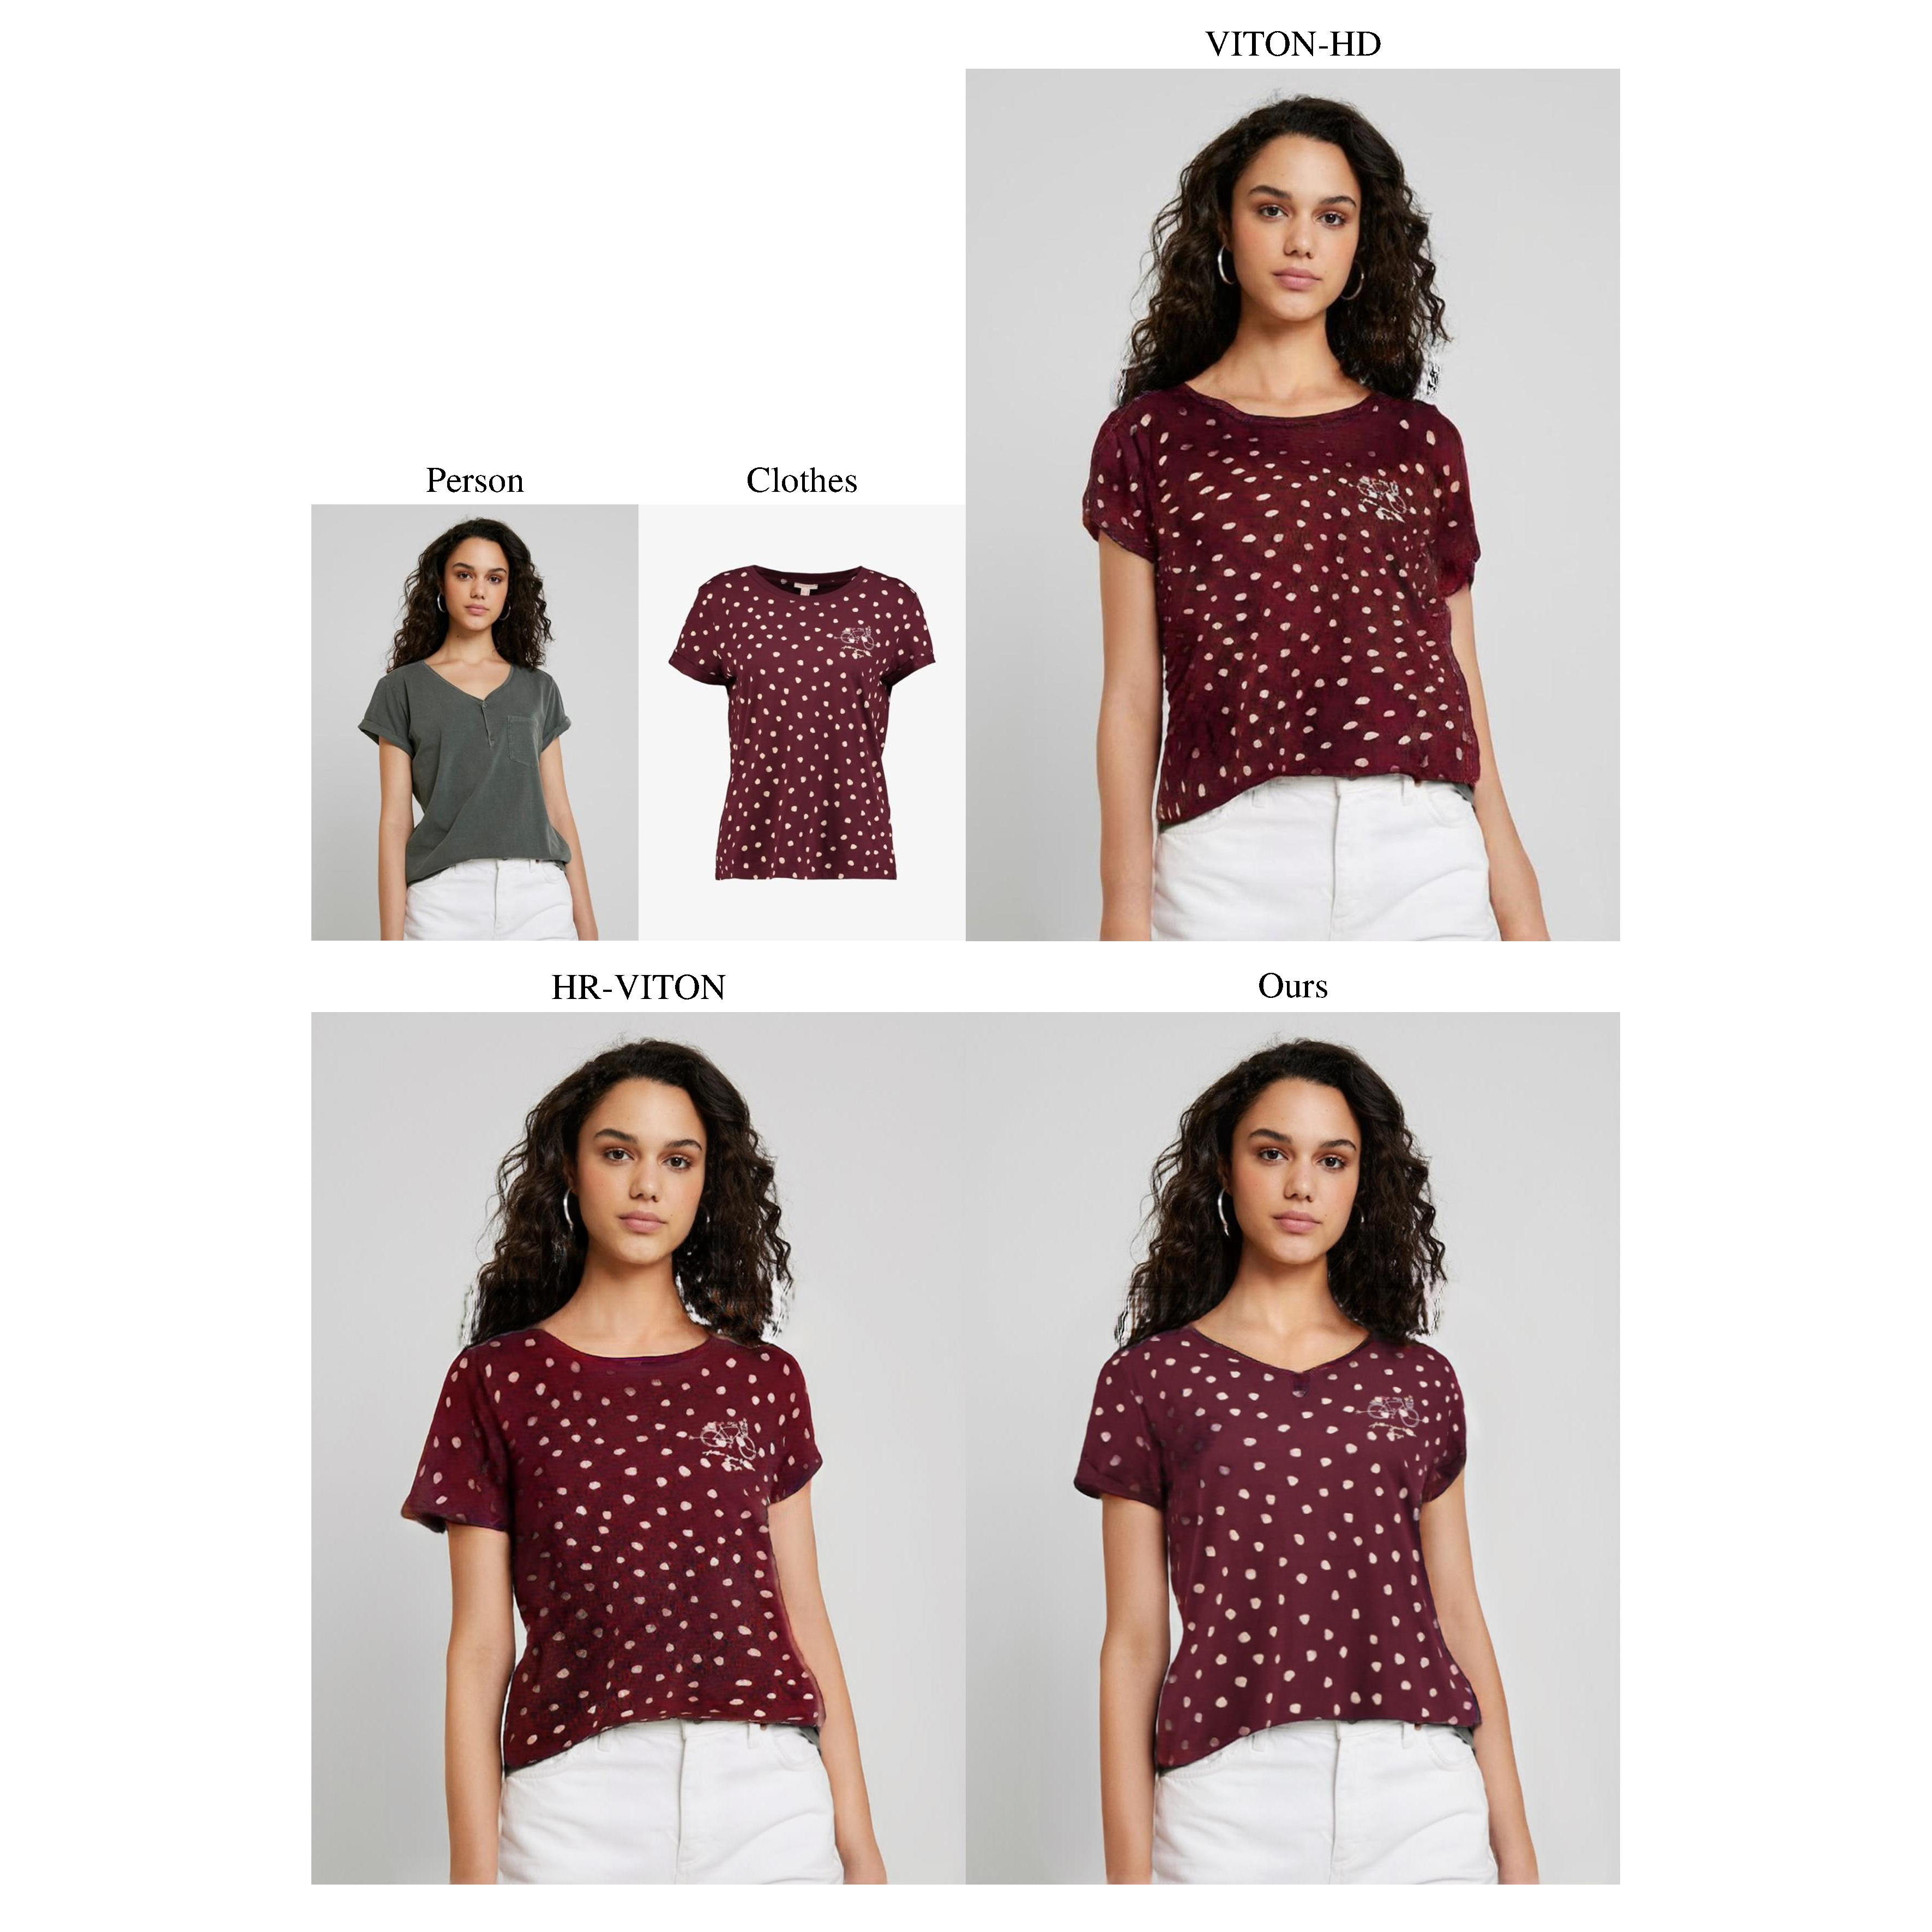
\includegraphics[width=0.85\textwidth]{fig_supp/fig_suppl_HD_11.pdf}
     \caption{Qualitative comparison between VITON-HD~\cite{choi2021viton}, HR-VITON~\cite{lee2022hrviton}, and ours. We recommend to look into the waist.
     }
     \label{fig_supp_tucked_in_HR_11}
\end{figure*}

